%% ----------------------------------------------------------------
%% Thesis.tex -- MAIN FILE (the one that you compile with LaTeX)
%% ---------------------------------------------------------------- 

% Set up the document
\documentclass[a4paper, 11pt, oneside]{Thesis}  % Use the "Thesis" style, based on the ECS Thesis style by Steve Gunn
\graphicspath{Figures/}  % Location of the graphics files (set up for graphics to be in PDF format)

% Include any extra LaTeX packages required

\usepackage{verbatim}  % Needed for the "comment" environment to make LaTeX comments
\usepackage{vector}  % Allows "\bvec{}" and "\buvec{}" for "blackboard" style bold vectors in maths
\usepackage[utf8]{inputenc}
\usepackage{subfiles} % access files in subdirectories
\usepackage{tabularx}
\usepackage{float}
\usepackage{amsmath}
\usepackage{csquotes}
\usepackage{listings}
\usepackage{fixltx2e}
\usepackage[english]{babel}
\usepackage{comment}
\usepackage{tikz}
\usepackage{hyperref}
\usepackage{glossaries}


\usepackage[
backend=biber,
style=ieee,
maxbibnames=99
]{biblatex}
\newcommand{\bibdirectory}{01_initial_try.bib}
\newcommand{\latex}{\LaTeX\xspace}
\newcommand{\tex}{\TeX\xspace}

%glossary making
\makeglossaries
% Example:
%\newglossaryentry{foobar}{%
%  name={Foobar},
%  description={A strange animal, not to be confused with \gls{foo}}
%}


\newglossaryentry{vector}{
    name={vector},
    description={An one-dimensional array of data}
}
\newglossaryentry{hyperparameters}{
    name={hyperparameters},
    description={A model hyperparameter is a configuration that is external to the model and whose value cannot be estimated from data.\parencite{brownlee_what_2017}}
}
\newglossaryentry{nonlinear}{
    name={nonlinear},
    description={The results of a function is unable to be reproduced from a linear combination of the inputs}
}
\newglossaryentry{layer}{
    name={layer},
    description={}
}
\newglossaryentry{InkML}{
    name={InkML},
    description={Ink Markup Language, defined by W3C. \parencite{chee_ink_2011}}
}
\newglossaryentry{WebSocket}{
    name={WebSocket},
    description={Enables event driven communication without. Client and server can push messages.}
}
\newglossaryentry{MVP}{
    name={MVP},
    description={Minimal viable product}
}
\addbibresource{\bibdirectory}
\hypersetup{urlcolor=blue, colorlinks=false, linkcolor=black}  % Colours hyperlinks in blue, but this can be distracting if there are many links.

%% ----------------------------------------------------------------

\begin{document}

\frontmatter      % Begin Roman style (i, ii, iii, iv...) page numbering
% Set up the Title Page
\title  {Recognition of handwritten mathematical symbols and expressions}
\authors {Even Dalen, Håvard Langdal and Torkil Solheim}
\addresses  {\groupname\\\deptname\\\univname}  % Do not change this here, instead these must be set in the "Thesis.cls" file, please look through it instead
\date       {\today}
\subject    {}
\keywords   {}

\maketitle
%% ----------------------------------------------------------------


\setstretch{1.3}  % It is better to have smaller font and larger line spacing than the other way round

% Define the page headers using the FancyHdr package and set up for one-sided printing
\fancyhead{}  % Clears all page headers and footers
\rhead{\thepage}  % Sets the right side header to show the page number
\lhead{}  % Clears the left side page header

\pagestyle{fancy}  % Finally, use the "fancy" page style to implement the FancyHdr headers


%% ----------------------------------------------------------------
% The preface page
\preface{
\addtocontents{toc}{\vspace{1em}}  % Add a gap in the Contents, for aesthetics

% Interesting assignment, machine learning, want to learn more
% Challenging
% New technology
% Curiosity




% Hvorfor ble oppgaven valgt
The assignment was chosen for several reasons. We were all interested in the contents of the assignment, and we saw this as a great opportunity to explore the machine learning world and learn new technologies. We had little to none prior experience with machine learning, and we knew this would be challenging. This however, made the assignment more interesting as we were motivated to learn and curious about ways to solve the problems related.

Before we chose the assignment, we read about the basics of neural networks and the mathematics behind them. We quickly understood that a lot of the math we have learned in previous courses was relevant, and being able to make use of this knowledge further increased our interest for the assignment. % siste setning må omformuleres muligens, litt bedre flyt, ellers kung

% Skriv kort om prosessen som har ført fram til resultatet.

%The process from start to finish was demanding. There have been days and even weeks where we felt no progress was made, which was frustrating and made us doubt our ideas.

% TODO PROCESS ER IKKE FERDIG!
The process from start to finish was demanding, we have had days, even weeks were we felt no progress was made. This is of course frustrating and made us doubt our ideas very often. In the initial phase of the project time went by much faster than expected, we spent several weeks just researching the most optimal way to solve the product part of our project. After the initial phase of the project we all had basic ideas about how it could be solved in the best way possible. % Nevne noen?
Although we had a lot of different ideas, we all quickly understood that in the first phase of coding, we should all use a method for high interaction and cooperation between us. This need of a solid method led us to pair programming, even though we were three. At first, this was extremely helpful, and it led to some creativity and a way to quickly respond to changes.
% 


% A lot of research
% Many ideas failed
% 

% Husk å takke for hjelp og støtte fra ulike hold
First of all, we would like to thank Ole Christian Eidheim for being both an inspiration and our mentor during this project. We would also like to thank our external mentors Tore Forbregd, Trygve Solstad and Hermund Andre Torkildsen for an exciting project and great inputs. %In addition to those respectable gentlemen, we would like to to mention CROHME, which has inspired our work and our thoughts on how to solve our assignment.


% Dette bør skrives om på hvis det skal brukes
%Through our (few) years at NTNU we have always had a facination for new technology, we always loved when our associate professor Ole Christian Eidheim just went on about whats the latest and hottest in computer science. It all eventually led to an class which introduced what machine learning is and what it hopes to accomplish, at that time we understood next to nothing. Our previous semester had a math heavy class which took us further into the world of numerical mathematics and other aspects. After reading about the project, and eventually about the basics of neural networks, we quickly understood that we could already make use of some of the knowledge acquired in this autumn. That, combined with the fact that this is something completely new for us and our curiosity made us choose this task. \\


%Dato, sted, navn og underskrift av alle prosjektdeltakerne.

\vfill

\begin{tabularx}{\textwidth}{XXX}
\centering{$\rule{4cm}{0.15mm}$} & \centering{$\rule{4cm}{0.15mm}$} & \centering{$\rule{4cm}{0.15mm}$} \tabularnewline
\centering{Even Dalen} & \centering{Håvard Langdal} & \centering{Torkil Solheim} \\
\end{tabularx}

\centering{\mydate}\\
\centering{Trondheim}

%Et forord i en rapport av denne typen bør ikke være på mer enn én side.

}

\clearpage  % Preface ended, start a new page

%% ----------------------------------------------------------------
% The Assignment page
\assignment{
\addtocontents{toc}{\vspace{1em}}  % Add a gap in the Contents, for aesthetics

%Erfaring viser at oppgavetekster endres underveis. Dere kan lime inn oppgaveteksten slik den var opprinnelig dersom det fortsatt er i samsvar med virkeligheten. Ellers gjør derekort rede for oppgaven slik den opprinnelig var,og slik den har utviklet seg underveis. Hvorfor ting har blitt som de har blitt, hører kanskje hjemme lenger ut i rapporten –det kommer litt an på hva det er.

\textit{
In this project, a handwriting recognition system for mathematical signs will be developed. The system will be used in a web application that is being developed at the Department of Teacher Education in collaboration with IDI. The system will use a standard machine learning algorithm such as convolutional neural networks that represent state-of-the-art handwriting recognition. Training data must be collected from students to train the network.
}

Since the beginning of the project, some changes were made to the assignment. Early on, it was not known if developing a system that would work well and enrich the functionality of the web application was actually achievable. Thus, there was decided to go in the direction of developing a proof of concept, which could be developed further. 

The assignment was also limited to focus on the handwriting recognition system, and not how to implement it into the web application.

What makes our schools bachelor's projects somewhat unique is the fact that we are in addition to solving an engineering task, we are also solving a hypothesis. At least that's the overall thought for software engineering projects, our project stands out as more of a research project than a pure software engineering project.



%The assignment quickly went in the direction of a proof of concept work, because it was not guaranteed that we would come up with something that would enrich the functionality of their current web application.
%In addition to this, the assignment was limited to focus on the handwriting recognition itself, and not all the possible ways to implement it into their web application. \\
%Nonetheless the assignment was challenging and finding a reasonable scientific problem related to the assignment was quite demanding. Especially if there was no direct correlation between the assignment and the scientific problem.
}
\clearpage % Assignment ended, start a new page 

%% ----------------------------------------------------------------

% The Abstract Page
\abstract{
\addtocontents{toc}{\vspace{1em}}  % Add a gap in the Contents, for aesthetics

In this thesis we researched different approaches for recognizing handwritten mathematical symbols and expressions. Interpreting different typographic styles has historically been a challenging task, however, recent improvements in both hardware and software for machine learning have made the task more approachable.

The purpose of the assignment was to create a module which interprets mathematical symbols and expressions. We created an example system to display how our module can be integrated into an independent system. Combined, the module and example system provide the complete functionality as specified by our project owners. 

Through our research, we explored different methods in pre- and post-processing of digital handwriting in order to best classify mathematical expressions. Our two approaches were to process drawings into images (using convolutional networks) and interpreting raw trace data (using recurrent networks). The combination of both approaches gave the best result and is the architecture used in our final model.
}

\clearpage  % Abstract ended, start a new page
%% ----------------------------------------------------------------

\setstretch{1.3}  % Reset the line-spacing to 1.3 for body text (if it has changed)

\pagestyle{fancy}  %The page style headers have been "empty" all this time, now use the "fancy" headers as defined before to bring them back


%% ----------------------------------------------------------------
\lhead{\emph{Contents}}  % Set the left side page header to "Contents"
\tableofcontents  % Write out the Table of Contents

%% ----------------------------------------------------------------
\lhead{\emph{List of Figures}}  % Set the left side page header to "List if Figures"
\listoffigures  % Write out the List of Figures

%% ----------------------------------------------------------------
\lhead{\emph{List of Tables}}  % Set the left side page header to "List of Tables"
\listoftables  % Write out the List of Tables


\lhead{\emph{List of Listings (Code and Snippets)}}
\lstlistoflistings
%% ----------------------------------------------------------------
%\setstretch{1.5}  % Set the line spacing to 1.5, this makes the following tables easier to read
\clearpage  % Start a new page



%% ----------------------------------------------------------------
%\clearpage  %Start a new page
%\lhead{\emph{Symbols}}  % Set the left side page header to "Symbols"
%\listofnomenclature{lll}  % Include a list of Symbols (a three column table)
%{
% symbol & name & unit \\
%$A$ & Matrix & \\
%$a$ & distance & m \\
%$P$ & power & W (Js$^{-1}$) \\
%& & \\ % Gap to separate the Roman symbols from the Greek
%$\omega$ & angular frequency & rads$^{-1}$ \\
%}
%% ----------------------------------------------------------------
% End of the pre-able, contents and lists of things
% Begin the Dedication page

%\setstretch{1.3}  % Return the line spacing back to 1.3


\addtocontents{toc}{\vspace{2em}}  % Add a gap in the Contents, for aesthetics


%% ----------------------------------------------------------------
\mainmatter	  % Begin normal, numeric (1,2,3...) page numbering
\pagestyle{fancy}  % Return the page headers back to the "fancy" style

% Include the chapters of the thesis, as separate files
% Just uncomment the lines as you write the chapters


% TODO; Make sure that the subdirectory can be compiled.
%\subfile{Chapters/Chapter1_Introduction}
\chapter{Introduction}
\lhead{\emph{Introduction}}  % Set the left side page header to "List if Figures"

\section{Motivation} % needs restructuring, we are finding out a way to combine cnn and rnn's, not develop 
% proof of concept++++++

Usage of digital tools in education is increasing, and testing student's performance is moving toward digital platforms. However, mathematics is a subject where most testing is still done on pen and paper. Few good digital tools exist for writing and validating mathematical handwritten expressions. By using machine learning to validate student's submission, the benefits of using digital tools for tests within the subject may improve, and therefore increase adoption of digital tools for mathematics.


%In education, the usage of digital tools has increased. In mathematics this is also true, but the digital tools in mathematics have been falling behind on some areas. Take GeoGebra for example, it is an amazing tool which fulfills your needs with style. What digital mathematics tools are missing is a way to provide input in more dynamic ways. % FUCK dette er vanskelig...


%In education the usage of digital tools to present and distribute tasks to students has increased [0]. % trenger kilde

%This includes tasks with multiple choice, graphs, geometric models and algebra. Traditionally these tools does not support dynamic input in form of digital ink, which makes the tools somewhat unrealistic from classic math on paper.

\section{Problem definition} 
\label{problem_definition}

Choosing a scientific problem or hypothesis turned out to be a challenge not knowing the potential of the assignment. Learning and experiencing from previous work on the same subject led us to explore the powers of a combination of convolutional and recurrent network.

How does a combination of recurrent and convolutional neural network's accuracy perform towards classifying handwritten mathematical symbols?

\section{Structure of the report}
\subsection{Chapter 1 Introduction}
The introduction consists of the motivation behind the project, the problem definition and some practical information about the thesis. In addition, a list of abbreviations is included at the end of the chapter.

\subsection{Chapter 2 Theory}
To understand this thesis and choices made, a lot of theory has to be understood. This chapter consists of relevant topics in handwriting recognition, machine learning and in general theoretical concepts needed to understand our work.

\subsection{Chapter 3 Technology and Method}
This chapter will specify the technology and how the technology is applied into our product. The purpose of this chapter is to give insight to how the results can be reproduced. Details about the different steps our recognition system undergoes is presented.

\subsection{Chapter 4 Results}
The results are divided into three parts:
\begin{enumerate}
    \item Scientific results
    
    This section will describe the results associated with the problem definition in section \ref{problem_definition}.
    
    \item Engineering results
    
    This section will describe the status of the system at the time of delivery and how the system fulfils the assignment.
    
    \item Administrative results
    
    This sections will discuss the goals in terms of project planning and how we managed time. In addition, how these goals changed accordingly to progress 
    
    The section will also contain how these goals changed accordingly to the continuous progress and the methodology used in the development.
    
\end{enumerate}

\subsection{Chapter 5 Discussion}
This chapter consist of discussion about the results and how they were achieved, the discussion is best described with questions. 
As well as possible future improvements to the system.

% vent med denne til vi har fylt kapitell 5 litt


\begin{enumerate}
    \item Scientific results
    An explanation of why or hypothesis did or did not hold, with focus on possible errors and areas of improvement.
    
    \item Engineering results
    An explanation of the software created in this project. Discussion about whether the system fulfils the product owners expectations.
    
    \item Administrative results
    Describe what went good or bad as a result of choosing a specific process, approach or technology. Including what went good or bad regardless of the chosen process, method or technology.
    
\end{enumerate}

\subsection{Chapter 6 Conclusion}
This chapter consists of our conclusion regarding our scientific problem and comments on further work.


\section{Target audience}
Machine learning is an extremely large field, with enormous potential. We encourage the reader to be open to some technical aspects including thoughts and choices made during the project. Machine learning is quite complex and we hope to inspire students and others new to machine learning. With that said, both our report and code is meant for a reader with some knowledge about software engineering, linear algebra and numerical mathematics. 

%Mye fra forrige avsnitt blir gjentatt her
%\subsection{Report} % Er dette et godt ord??
%This project report is meant for everyone curious about an specific introduction to practical examples of machine learning using neural networks. The specific part is linked to this projects assignment, which is to use different approaches to achieve an respectable accuracy.\\
% line break
%Even though this report is meant as an introduction to a complicated field, we have based our writing on that the reader has knowledge equivalent to an 2nd year computer engineering student at Norwegian University of Science and Technology in Trondheim. Thus, some of the fundamentals are excluded. % ok setning?


\subsection{Application}
The application consists of an simple back end and a front end library and is available to use under the MIT license \cite{_mit_????}. As previously stated, the application is specifically created to fit the needs of our product owners, however, the front end library can be used in a more general matter. % TODO bruk bilder, figurer eller lignende av applikasjonen (?)


%\section{CROHME} % Teori
%CROHME is an abbreviation for Competition on Recognition of Online Handwritten Mathematical Expressions.
%CROHME is a competition for recognizing online handwritten mathematical symbols. CROHME is organized by International Conference on Frontiers in Handwriting Recognition. \\ 
%CROHME 2016 \parencite{mouchere_icfhr2016_2016} concluded with that handwriting is still a challenge to be solved, even after six years of competitions. Ratings on the individual tasks was accomplished, but overall it requires first of all, the segmentation to be perfect. An error in the segmentation process will supply the next steps with incorrect information and a bad foundation to perform classification on.
% si noe om "junk" ? filtrering osv er ikke lett
%The winner of CROHME 2016 and other competition years, was MyScript. MyScript has a commercial solution which has rich functionality and good results, but they managed to achieve those results with their own private data set. \parencite{mouchere_icfhr2016_2016}  \\ 

%Tror egt ikke vi trenger den her, vi kan prøve å flette den litt sammen med motivation
\section{Purpose}
The purpose of this project is both to create something useful for our product owners, while exploring the possibilities and limitations of recognition of handwritten mathematical symbols. In addition, we hope to inspire further work on the subject. 

%Litt rart og ha det her under purpose
Choices made during the project were strongly influenced by previous work, for example Martin Thoma, 2015 \cite{thoma_-line_2015} and Catherine Lu and Karanveer Mohan \cite{lu_recognition_2015}.

\section{Abbreviations}  % Set the left side page header to "Abbreviations"
\begin{table}[H]
\begin{tabular}{ l l }
\textbf{ANN} & Artificial Neural Network \\
\textbf{BMP} & Bitmap \\
\textbf{CNN} & Convolutional Neural Network \\
\textbf{CPU} & Central Processing Unit \\
\textbf{CROHME} & Competition on Recognition of Online Handwritten Mathematical Expressions\\
\textbf{CSS} & Cascading Style Sheets \\
\textbf{GPU} & Graphics Processing Unit \\
\textbf{GUI} & Graphical User Interface \\
\textbf{HTML} & HyperText Markup Language \\ 
\textbf{ICFHR} & International Conference on Frontiers in Handwriting Recognition \\
\textbf{IDE} & Integrated Development Environment \\
\textbf{ILU} & Department of Teacher Education \\
\textbf{InkML} & Ink Markup Language \\
\textbf{JSON} & JavaScript Object Notation \\
\textbf{LSTM} & Long Short-Term Memory \\
\textbf{MLP} & Multilayer Perceptrons \\
\textbf{MNIST} & Modified National Institute of Standards and Technology database \\
\textbf{NTNU} & Norwegian University of Science and Technology \\
\textbf{OCR} & Optical Character Recognition \\
\textbf{RDP} & Ramer-Douglas-Peucker algorithm \\
\textbf{RNN} & Recurrent Neural Network \\
\textbf{GRU} & Gated Recurrent Unit \\
\textbf{LSTM} & Long Short-Term Memory \\

\end{tabular}
\label{table:abbreviations}
\caption{A list of abbreviations used, in alphabetical order.}
\end{table}

\chapter{Theory}
\lhead{\emph{Theory}}
% TODO CITE
% KERAS
% SKLEARN
% NUMPY

\section{Handwriting recognition}
\label{handwriting_recognition}

Handwriting recognition systems are computer systems that can recognize characters and symbols written by hand. These systems have been continuously developed and researched since the early days of computers \cite{simon_off-line_1992}, beginning with the optical character recognition (OCR) systems in the 1950s \cite{mori_historical_1992}. The early OCR systems were very limited in terms of hardware, which resulted in slow progress. Researchers had high aspirations for handwriting recognition, however, it quickly gained the reputation of being an extremely difficult problem \cite{simon_off-line_1992}. As hardware and computers became more advanced, the OCR and handwriting recognition systems followed in the same direction. However, hardware has often been a bottleneck for these systems \cite{mori_historical_1992}.

When computational power increased, using artificial neural networks became more popular, also for handwriting recognition. For example, in \cite{fukushima_handwritten_????} by Fukushima et al., a neural network was trained to recognize 35 symbols. Since then, neural networks has been used in many solutions, and has proven to be a major contributor to the field, as it is one of the most used tools in leading solutions today (some of these are presented in section \ref{previous_work_existing_solutions}).

This field has for a long time been a worldwide research project \cite{mori_historical_1992}, and many competitions on different handwriting recognition problems has been arranged. Researchers from all over the world has cooperated to produce various solutions, which further confirms the difficulty of a general handwriting recognition system. 

\subsection{Main approaches}
\label{main_approaches}

Handwriting recognition systems generally has two main approaches, online and offline \cite{priya_online_2016}. Online recognition uses data from pen strokes based on sampled coordinates of pen movements and the time difference between them. These pen strokes are also referred to as traces.  Each trace can be uniquely identified while drawing, which in many cases can aid in the segmentation problem (see section \ref{Segmentation}).

While online recognition uses sequential data, offline recognition uses images. In this approach the recognition system relies solely on the pixel values in images. Traces can therefore not be uniquely identified, as opposed to online recognition.


\begin{figure}[H]
\centering
\begin{subfigure}{0.3\textwidth}
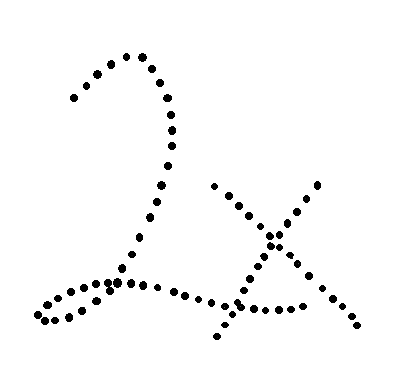
\includegraphics[width=1.1\linewidth, height=5cm]{Assets/Chapter2_Theory/segmentation_2_on.png} 
\caption{}
\label{fig:online_data}
\end{subfigure}
\begin{subfigure}{0.3\textwidth}

\includegraphics[width=1.1\linewidth, height=5cm]{Assets/Chapter2_Theory/segmentation_2.png}
\caption{}
\label{fig:offline_data}
\end{subfigure}
\caption{A: Online input data with coordinate samples. B: Offline input data (only an image).}
\label{fig:online_offline_comparison}
\end{figure}

With the online input data, creating images of the traces is possible by drawing lines between the coordinates. This means that online recognition systems has access to roughly the same images as offline recognition systems, in addition to the coordinates. Having more features to analyze is important since handwriting styles can vary a lot. In general, online recognition systems has higher performance and accuracy than offline recognition systems \cite{priya_online_2016}.

\subsection{Common steps in handwriting recognition}

\subsubsection{Preprocessing}

In the preprocessing step the raw input data is prepared for analysis. Raw input data can come in many formats and sizes, and may contain values that are not valid. This step deals with these problems and converts the data to a format that suits the consecutive steps better. To further optimize the flow, excess data can be discarded \cite{huang_preprocessing_2007}.

A common task in preprocessing is to normalize the input data. This simply means that all the data is scaled to the same value range, to eliminate deviations. For handwriting recognition, normalizing generalizes the different writing styles by removing some of the variations \cite{huang_preprocessing_2007}.

Since the input can be offline or online, there are many techniques that can be used to prepare the data. Common tasks in preprocessing of offline data includes removal of noise from the images and converting greyscale images to binary images \cite{priya_online_2016}. The images could also be scaled and modified to not contain any blank or empty space.

Online data can be processed in different ways than offline data. For example, the coordinates can be plotted and lines can be drawn between them. This is often called a polygonal chain. Without any preprocessing these plots can have sharp edges and overall be a inaccurate representation of handwriting. Smoothing could be applied to the coordinates to fix this by using interpolation of points. The data samples might also need to be parsed to a format that is more suitable for processing, such as matrices or arrays.

To normalize traces to have the same number of data points, a variation of the Ramer-Douglas-Peucker (RDP) \cite{h_algorithms_2011} algorithm can be used. The RDP algorithm attempts to simplify a polygonal chain, while minimizing the difference between the original and the simplified chain. The simplification process works by finding data points which influences the shape of the chain less than a fixed threshold.

The algorithm can be modified to decrease the number of data points to a fixed number. This can be done by iterating all the data points three at a time, and removing the middle point with lowest perpendicular distance to a line drawn between the two endpoints.

\begin{figure}[H]
    \centering
    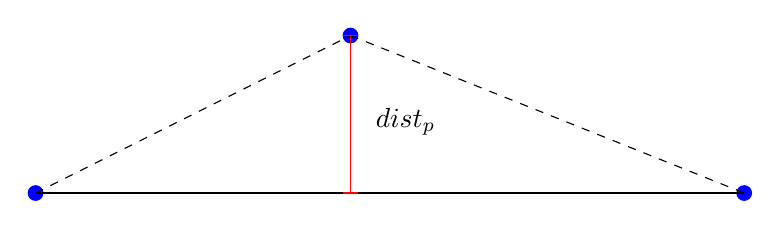
\begin{tikzpicture}
    
        %Datapoints
        \fill[blue] (-3, 0) circle (0.1cm);
        \fill[blue] (1, 2) circle (0.1cm);
        \fill[blue] (6, 0) circle (0.1cm);

        \draw[-] (-3, 0) -- (6, 0);
        \draw[dashed] (-3,0) -- (1, 2);
        \draw[dashed] (1, 2) -- (6, 0);
        
        \draw[red, -] (1, 2) -- (1, 0);
        \draw[red, -] (0.9, 2) -- (1.1, 2);
        \draw[red, -] (0.9, 0) -- (1.1, 0);
        \node at (1.7, 0.9) {$dist_p$};

    \end{tikzpicture}
    \caption{Figure of calculating the perpendicular distance to a line drawn between two endpoints}
    \label{fig:my_label}
\end{figure}
\label{ramer_douglas_peucker}

In order to normalize traces from different sources, their coordinates needs to be scaled within the same range. A maximum and and minimum value, the roof and floor of the range specified, is used together with a list of x- or y-coordinates.

First, the maximum and minimum values of the list are found, as well as the difference between them. The scaled values are then found with this formula \cite{_normalize_????}:

\begin{equation} \label{eqn:scale_linear_by_column}
\centering
\begin{split}
    s = roof - \frac{(roof - floor) \cdot (max(x) - x)}{diff}
\end{split}
\end{equation}
\label{scale_linear_by_column}

\subsubsection{Segmentation} \label{Segmentation}

The segmentation problem deals with extraction of symbols from trace-coordinates or images. Deciding if two traces that overlap belongs to the same symbol is difficult, since they can overlap in countless ways. 

\begin{figure}[H]
\centering
\begin{tikzpicture}
\begin{scope}[xshift=1.5cm]
    \node[anchor=south west,inner sep=0] (image) at (0,0) {
\includegraphics[width=0.2\textwidth]{Assets/Chapter2_Theory/segmentation_2.png}};
    \begin{scope}[x={(image.south east)},y={(image.north west)}]
        \draw[->] (1,0.5) -- (1.9,0.8);
        \draw[->] (1,0.4) -- (1.9,0.4);
        \draw[->] (1,0.3) -- (1.9,0);
        \node [anchor=west] (note) at (2,0.9) {\Large 2x};
        \node [anchor=west] (note) at (2,0.4) {\Large $\Delta$};
        \node [anchor=west] (note) at (2,-0.1) {\Large 2/\textbackslash};
        \node [anchor=west] (note) at (2.4,0.4) {\Huge ?};
    \end{scope}
\end{scope}
\end{tikzpicture}
\caption{The segmentation problem deals with extraction of symbols from trace-coordinates or images. The sample above has three traces, one for the "2"  and two for the "x". How they are segmented can lead to many different outcomes.}
\label{fig:segmentation_1}
\end{figure}

Correctly segmenting the symbols is important for the recognition process since it heavily affects the final results. A simple way of dealing with the problem with online data is to merge the traces that overlap to a single symbol. In this case the sample above would combine the '2' and the 'x' to a single symbol, which would lead to a wrong classification. A more complicated approach is presented in \cite{nguyen_improved_2015} where a bidirectional long-short term memory neural network (see section \ref{theory-LSTM}) is used to segment English handwritten text.

% BOUNDING BOXES
Segmentation could also be solved with object detection using bounding boxes. Bounding boxes encapsulates the search range of a given symbol in order to correctly extract its underlying data. A bounding box consist of four numbers specifying its width, height and starting point.


% Kanskje legge inn noe her om at preprosessering og segmentering er tett knyttet sammen, ikke pri

\subsubsection{Classification of symbols}
The classification step deals with the actual recognition. In this step each of the segmented symbols are classified. As the number of classes increases, the recognition rates typically drops since the system has to distinguish between more types of symbols.

A popular approach for this is to use neural networks (see section \ref{artificial_neural_networks}). For image classification, neural networks has achieved very high rates and is regarded as the current state-of-the-art algorithm \cite{seif_deep_2018}.

\subsubsection{Postprocessing}

After the classification the results can be further analyzed and converted to the desired format. In \cite{hu_research_2011}, a dictionary based postprocessing method is used to improve the recognition results by checking if the classification results are valid. With a dictionary, the recognition system can filter out words that does not exist, and replace them with similar and valid words. 

Another way to further improve the results is to use contextual analysis. With this approach the positions of the input data is analyzed with regards to the classification results. Grammatical errors and results that does not make sense might be revealed, and can be used to trigger a re-classification with the last results in mind.


\section{Recognition of handwritten mathematics} 
\label{recognition_of_handwritten_mathematics}
Recognition of handwritten mathematics is a field in handwriting recognition that deals with mathematical symbols and expressions. This field shares many of the same problems as recognition of words and characters, however, there is also a new problem that must be dealt with. Just as regular language, mathematics has a set of grammatical or positional rules that should be followed. For example, there are fractions, exponents and square roots that has to be interpreted correctly. This two-dimensional notation requires further processing techniques compared to analyzing regular words.

A context of how all the symbols fit together has to be built by looking at positional values. This context search could be done in the post-processing step, using the results of the classification for guidance. The classification of symbols might also be completely wrong, as the truth to a symbol has many context-dependencies \cite{zanibbi_recognition_2012}. For instance, the decimal separator "." and the multiplication operator "$\cdot$" must be interpreted based on their position to their surroundings. 

\begin{figure}[H]
\centering
    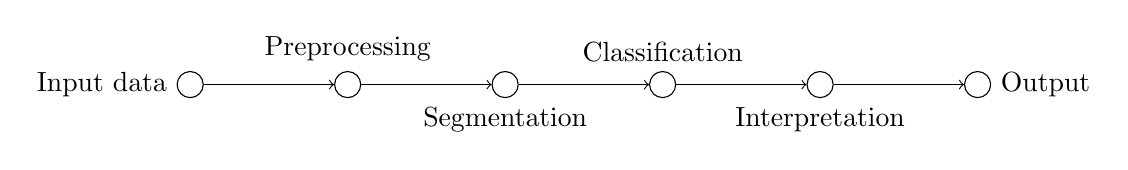
\begin{tikzpicture}[->,',auto,node distance=2cm,main node/.style={circle,draw},sub node/.style={draw}]
    \node[main node] (1) [label=left:Input data] {};
    \node[main node] (2) [label=above:Preprocessing, right of=1] {};
    \node[main node] (3) [label=below:Segmentation, right of=2] {};
    \node[main node] (4) [label=above:Classification, right of=3] {};
    \node[main node] (5) [label=below:Interpretation, right of=4] {};
    \node[main node] (6) [right of=5,label=right:Output] {};

    \path[every node/.style={font=\sffamily\small}]
        (1) edge node [right] {} (2)
        (2) edge node [right] {} (3)
        (3) edge node [right] {} (4)
        (4) edge node [right] {} (5)
        (5) edge node [right] {} (6);

    \end{tikzpicture}
    \caption{Steps in recognition of mathematical expressions.}

\label{fig:steps_in_math_recog}
\end{figure}

\subsection{Previous work and existing solutions}
\label{previous_work_existing_solutions}
There is a lot of work previously done in recognition of handwritten mathematics, and many solutions has been made. The first work in this field dates back to the 60s and has gradually developed since \cite{mouchere_icfhr2016_2016}. Different solutions and ideas has been presented through many publications from all over the world. For example, in \cite{matsakis_recognition_????} from 1999, a system that uses a Gaussian classifier for recognition of handwritten mathematics is demonstrated.

In recent years a competition called \textit{Competition on Recognition of Online Handwritten Mathematical Expressions} hosted by ICFHR has been held \cite{mouchere_icfhr2016_2016} \cite{mouchere_advancing_2016}. In these competitions teams from around the world competed in various math recognition tasks. The main task was to recognize expressions, while subtasks for example was to recognize matrices and isolated symbols. This competition has contributed a lot to the math recognition field, by producing standardized data sets and evaluation metrics.

In the CROHME competition held in 2016 the MyScript corporation won in all categories. To produce the best results, their system handles segmentation, classifying and interpretation concurrently. The system uses features from both bitmaps and digital ink traces that are sent through a combination of MLP and recurrent neural networks \cite{mouchere_icfhr2016_2016}. As of \mydate their technology is commercially available.

\subsection{InkML}
InkML is a markup language based on XML to describe digital ink data. The format is specified by the World Wide Web Consortium (W3C) \cite{chee_ink_2011}. InkML groups it's content in specific XML-style elements called ink. These elements contains trace elements, which stores coordinates for the traces. 

\begin{figure}[H]
\begin{lstlisting}[language=XML]
<trace id="0">
    207 136, 199 141, 197 143, 196 144, 195 146, 194 147, 193 149
</trace>
<trace id="1">
    847 201, 847 204, 846 207, 846 211, 846 215, 845 219, 845 222
</trace>
<trace id="2">
    833 235, 822 235, 821 235, 820 235, 819 236, 819 235, 819 236
</trace>

<traceGroup xml:id="3">
	<annotation type="truth">+</annotation>
	<traceView traceDataRef="1"/>
	<traceView traceDataRef="2"/>
	<annotationXML href="+_1"/>
</traceGroup>
\end{lstlisting}

\caption{InkML example of three traces, each with an file-unique id. In addition to traces, a trace group is included to connect truths to traces. Truths are used when providing labels to use in supervised learning, and is explained in section \ref{supervised_learning}.}

\label{fig:InkML_ex}
\end{figure}

\section{Machine learning}
\label{machine_learning}
According to Murphy et al.\cite{murphy_machine_2012}, machine learning can be defined as a set of methods that can automatically detect patterns in data. These uncovered patterns can also be used to predict future data or support decision making. For example, historical data of maintenance can be used to predict failure for individual mechanical parts \cite{cline_predictive_2017}. Goodfellow et al. explains machine learning as an applied form of statistics \cite{goodfellow_deep_2016}.

\subsection{Supervised learning}
\label{supervised_learning}

Supervised learning is the machine learning task to map an input to an output. It requires large amounts of training data, with features and an additional truth label.

A supervised learning algorithm can study examples of the classification tasks, often referred to as training data. Eventually the algorithm will learn features common to each class, and thereby be able to classify unseen data. To explain this in another way think of the function p(y $|$ x), this reads the probability of y given x has happened. This is exactly what supervised learning is, where the y labels are provided by a supervisor.

\section{Artificial neural networks}
\label{artificial_neural_networks}

Artificial neural network (ANN) is a subset of supervised learning algorithms. These are algorithms inspired by biological neural networks.

ANNs consists of a combination of artificial neurons, also referred to as computational units. These units takes a vector as input. The input is multiplied with the precomputed weights, and a bias is added. A bias is used in the same way as the constant b in the equation $y = ax + b$, in order to shift the function up or down. Then, the result is summed and used as input to the activation function \ref{activation_functions}. Lastly, the weighted sum is returned as output from the unit \cite{_cs231n_????} \cite{_multi-layer_????}.

\begin{figure}[H]
  \centering
    \begin{tikzpicture}
        \draw[->] (0,2) -- (2.1,0.8);
        \draw[->] (0,0.65) -- (2,0.3);
        \draw[->] (0,-0.65) -- (2,-0.3);
        \draw[->] (0,-2) -- (2.1,-0.8);
    
        \node at (0.2, 2.3) {$x_1$};
        \node at (0.2, 1) {$x_2$};
        \node at (0.2, -0.25) {$...$};
        \node at (0.2, -1.5) {$x_n$};
        
        \draw [] (4.2,0) ellipse (2cm and 1cm);
        
        \node at (4.2,0) {$\sum\limits_{i=1}^{n} W_i \cdot x_i + b$};
        
        \draw[->] (6.5,0) -- (7.5,0);
        
        \draw (7.8, 0.8) rectangle (9.8, -0.8);
    
        \node at (8.8,0) {$f : R \rightarrow R$};
    
    \end{tikzpicture}
    \caption{Diagram of a single artificial neuron. $W_{i}$ is the weight of input edge i, $x_{i}$ is the value coming from edge i and b is the bias.} % TODO denne trenger mer kjøtt, god forklaring fra a til å!
    \label{fig:single_neuron}

\end{figure}

The units in a neural network are typically organized into different layers, where each layer has a fixed number of units. The diagram below is an example of how these units can be connected together.

\begin{figure}[H]
  \centering

    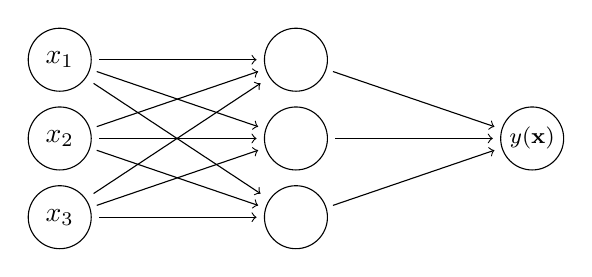
\begin{tikzpicture}
        
        \draw [] (0.5,1) circle [radius=0.4];
        \draw [] (0.5,0) circle [radius=0.4];
        \draw [] (0.5,-1) circle [radius=0.4];

        \draw [] (3.5,1) circle [radius=0.4];
        \draw [] (3.5,0) circle [radius=0.4];
        \draw [] (3.5,-1) circle [radius=0.4];

        \draw [] (6.5, 0) circle [radius=0.4];

        \draw[->] (1,1) -- (3,1);
        \draw[->] (0.97,0.85) -- (3.02,0.15);
        \draw[->] (0.93,0.7) -- (3.05,-0.7);

        \draw[->] (0.97,0.15) -- (3.02,0.85);
        \draw[->] (1,0) -- (3,0);
        \draw[->] (0.97,-0.15) -- (3.02,-0.85);

        \draw[->] (0.93,-0.7) -- (3.05,0.7);
        \draw[->] (0.97,-0.85) -- (3.02,-0.15);
        \draw[->] (1,-1) -- (3,-1);
        
        \draw[->] (3.97,0.85) -- (6.02,0.15);
        \draw[->] (4, 0) -- (6,0);
        \draw[->] (3.97, -0.85) -- (6.02,-0.15);

        \node at (0.5,1) {$x_1$};
        \node at (0.5,0) {$x_2$};
        \node at (0.5,-1) {$x_3$};
        \node at (6.5,0) {\footnotesize$y(\textbf{x})$};

    \end{tikzpicture}
    \caption{Diagram of a neural network with two layers (Output layer and one hidden layer). It contains three units in the input layer, three units in the hidden layer, and a single unit in the output layer. }
    \label{fig:single_layered_neural_network}
\end{figure}


The leftmost layer of units in \ref{fig:single_layered_neural_network} is called the input layer, and is a passive layer. This means that data is not modified in this layer. Each unit in the input layer receives a single input and duplicate the input to its multiple output units. The hidden layer and the output layer from \ref{fig:single_layered_neural_network} are active units. These units modify the data before propagating the values to the next layer (described in \ref{fig:single_neuron}). The result of the output layer is the approximation done by the neural network \parencite{smith_scientist_1997}. 

In order for a neural network to be a good approximator, the weights and biases in each unit has to be optimized to minimize error in the output layer. This tuning process is performed through training. Training a network means giving the network labeled training data, comparing the output label from the network to the label provided, and tuning the weights and biases to best satisfy a loss function (\ref{loss_function}). This optimization process is typically done using an optimizer such as gradient decent, and through a concept called backpropogation. This is described in section \ref{training_with_backpropagation}.

% THIS SECTION IS PREVIOUSLY CALCULATING AN OUTPUT
The output of a neural network is a set of numerical values, one value for each of the output units in the neural network. To create these output values the neural network performs a series of mathematical operations on the input values.
%The output of a neural network is a vector of numerical values. This vector contains as many values as there are output units in the neural network. To create this output vector the neural network performs a series mathematical operations on the input vector. 

For this demonstration the network in figure \ref{fig:single_layered_neural_network} will be used. The first step is to calculate the outputs from the hidden layer, $H_o$.
\begin{figure}[H]
  \centering

    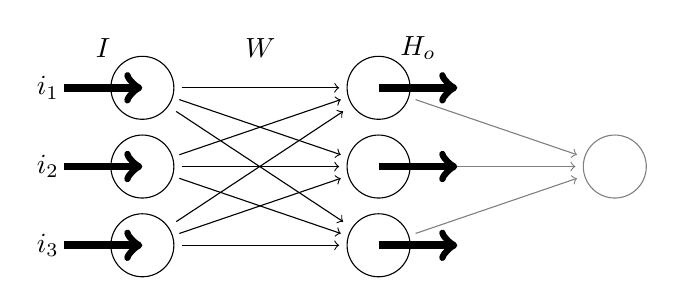
\begin{tikzpicture}
        
        \draw [] (0.5,1) circle [radius=0.4];
        \draw [] (0.5,0) circle [radius=0.4];
        \draw [] (0.5,-1) circle [radius=0.4];

        \draw [] (3.5,1) circle [radius=0.4];
        \draw [] (3.5,0) circle [radius=0.4];
        \draw [] (3.5,-1) circle [radius=0.4];

        \draw [draw={rgb:black,2;white,2}] (6.5, 0) circle [radius=0.4];

        \draw[->] (1,1) -- (3,1);
        \draw[->] (0.97,0.85) -- (3.02,0.15);
        \draw[->] (0.93,0.7) -- (3.05,-0.7);

        \draw[->] (0.97,0.15) -- (3.02,0.85);
        \draw[->] (1,0) -- (3,0);
        \draw[->] (0.97,-0.15) -- (3.02,-0.85);

        \draw[->] (0.93,-0.7) -- (3.05,0.7);
        \draw[->] (0.97,-0.85) -- (3.02,-0.15);
        \draw[->] (1,-1) -- (3,-1);
        
        \draw[draw={rgb:black,2;white,2}, ->] (3.97,0.85) -- (6.02,0.15);
        \draw[draw={rgb:black,2;white,2}, ->] (4, 0) -- (6,0);
        \draw[draw={rgb:black,2;white,2}, ->] (3.97, -0.85) -- (6.02,-0.15);

        %\node at (0.5,1) {$x_1$};
        %\node at (0.5,0) {$x_2$};
        %\node at (0.5,-1) {$x_3$};
        %\node[text={rgb:black,2;white,2}] at (6.5,0) {\footnotesize$y(\textbf{x})$};
        
        \draw[->, line width=1mm] (3.5,1) -- (4.5,1);
        \draw[->, line width=1mm] (3.5,0) -- (4.5,0);
        \draw[->, line width=1mm] (3.5,-1) -- (4.5,-1);
        
        \draw[->, line width=1mm] (-0.5,1) -- (0.5,1);
        \draw[->, line width=1mm] (-0.5,0) -- (0.5,0);
        \draw[->, line width=1mm] (-0.5,-1) -- (0.5,-1);
        
        \node at (0,1.5) {$I$};
        \node at (-0.7,1) {$i_1$};
        \node at (-0.7,0) {$i_2$};
        \node at (-0.7,-1) {$i_3$};
        
        \node at (2,1.5) {$W$};
        \node at (4,1.5) {$H_o$};
        
        

    \end{tikzpicture}
    \caption{The outputs of the hidden layer is calculated based on the inut values and the weights between the input layer and hidden layer.}
    \label{fig:calculating_output_one}
\end{figure}

Each of the input values are multiplied with the weight to each unit in the hidden layer. All the inputs to a unit in the hidden layer is then summed. Matrix multiplication can be used for this, where a matrix containing all the weights is multiplied with a column-matrix containing the input values. The weights matrix in this example is a 3x3 matrix since there are 3 inputs and 3 units in the hidden layer.

\begin{center}
$
W * I = 
\begin{bmatrix} 
w_{1,1} & w_{2,1} & w_{3,1}\\
w_{1,2} & w_{2,2} & w_{3,2}\\
w_{1,3} & w_{2,3} & w_{3,3}
\end{bmatrix}
*
\begin{bmatrix} 
i_1\\
i_2\\
i_3
\end{bmatrix}
=
\begin{bmatrix} 
h_1\\
h_2\\
h_3
\end{bmatrix}
=
H_i
$
\end{center}

To calculate the output from the hidden layer an activation function is used on these input values: $activation(H_i) = H_o$. More details about activation functions is explained in section \ref{activation_functions}.

%\begin{center}
%$
%activation(H_i) = H_o
%$    
%\end{center}

The output from the hidden layer is then sent further in the network.

\begin{figure}[H]
  \centering

    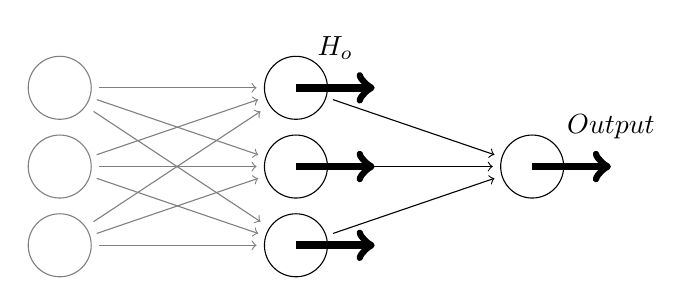
\begin{tikzpicture}
        
        \draw [draw={rgb:black,2;white,2}] (0.5,1) circle [radius=0.4];
        \draw [draw={rgb:black,2;white,2}] (0.5,0) circle [radius=0.4];
        \draw [draw={rgb:black,2;white,2}] (0.5,-1) circle [radius=0.4];

        \draw [] (3.5,1) circle [radius=0.4];
        \draw [] (3.5,0) circle [radius=0.4];
        \draw [] (3.5,-1) circle [radius=0.4];

        \draw [] (6.5, 0) circle [radius=0.4];

        \draw[draw={rgb:black,2;white,2}, ->] (1,1) -- (3,1);
        \draw[draw={rgb:black,2;white,2}, ->] (0.97,0.85) -- (3.02,0.15);
        \draw[draw={rgb:black,2;white,2}, ->] (0.93,0.7) -- (3.05,-0.7);

        \draw[draw={rgb:black,2;white,2}, ->] (0.97,0.15) -- (3.02,0.85);
        \draw[draw={rgb:black,2;white,2}, ->] (1,0) -- (3,0);
        \draw[draw={rgb:black,2;white,2}, ->] (0.97,-0.15) -- (3.02,-0.85);

        \draw[draw={rgb:black,2;white,2}, ->] (0.93,-0.7) -- (3.05,0.7);
        \draw[draw={rgb:black,2;white,2}, ->] (0.97,-0.85) -- (3.02,-0.15);
        \draw[draw={rgb:black,2;white,2}, ->] (1,-1) -- (3,-1);
        
        \draw[->] (3.97,0.85) -- (6.02,0.15);
        \draw[->] (4, 0) -- (6,0);
        \draw[->] (3.97, -0.85) -- (6.02,-0.15);

        \draw[->, line width=1mm] (3.5,1) -- (4.5,1);
        \draw[->, line width=1mm] (3.5,0) -- (4.5,0);
        \draw[->, line width=1mm] (3.5,-1) -- (4.5,-1);
        
        \draw[->, line width=1mm] (6.5,0) -- (7.5,0);
        
        \node at (4,1.5) {$H_o$};
        \node at (7.5,0.5) {$Output$};

    \end{tikzpicture}
    \caption{The final output is calculated}
    \label{fig:calculating_output_two}
\end{figure}
The same matrix and activation function calculation is then repeated. However, now performed on the output from the hidden layer and the weight to the output layer. This will calculate the final output from the neural network. Since the output layer consist of only one unit, the final output will be a single value.

For a larger neural network the same process is used but on a bigger scale. If a neural network has more than a single hidden layer, the process is repeated for each of the layers.




\subsection{Activation functions} % TODO  trim dette litt ned, siden core concepts tar for seg basics.
\label{activation_functions}

Activation functions in artificial neural networks has inspiration from how neurons in our brain works. In a mathematical model of an artificial neuron by McCulloch-Pitt \cite{mcculloch_logical_1943}, the activation of a neuron was modelled as the unit step function. This model has later been generalized to use functions such as sigmoid, rectified linear unit, softmax and tangens hyperbolicus \cite{jain_artificial_1996}.

\begin{figure}[H]
  \centering
    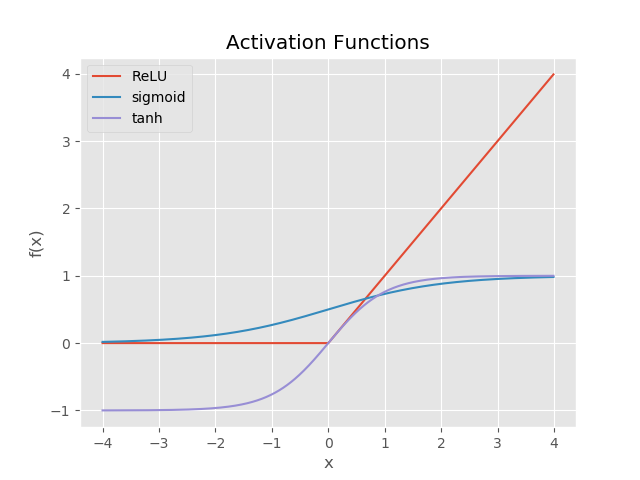
\includegraphics[width=0.9\textwidth]{Assets/Chapter2_Theory/activation_function_overview.png}
    \caption{Three activation functions plotted on the interval [-4,4].}
\end{figure}

One purpose of an activation function is to introduce nonlinearity into the model. A network without nonlinearity can't represent functions which are nonlinear, despite having multiple layers. On the other hand, it is proved that a multilayered feedforward network with nonlinear activation functions can approximate any function (under some constraints) \cite{leshno_multilayer_1993}.

 An example of the importance of nonlinearity in neural networks can shown in the exclusive-OR problem illustrated in the figure below. The black dots can not be separated from the white using a single line. On the other hand, a combination of nonlinear functions can create arbitrary shapes to separate the white and black dots \cite{jain_artificial_1996} \cite{sharma_understanding_2018}.

\begin{figure}[H]
  \centering

    \begin{subfigure}{.45\textwidth}
      \centering

        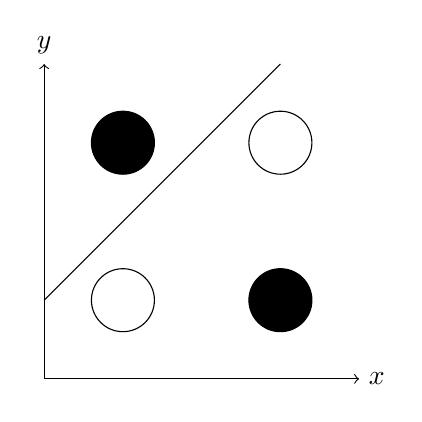
\begin{tikzpicture}
        
            \draw [fill=black] (0.5,1) circle [radius=0.4];
            \draw [] (0.5,-1) circle [radius=0.4];
    
            \draw [] (2.5,1) circle [radius=0.4];
            \draw [fill=black] (2.5,-1) circle [radius=0.4];
    
            \draw[-] (-0.5, -1) -- (2.5,2);
    
            \draw[->] (-0.5,-2) -- (3.5,-2) node[right] {$x$};
            \draw[->] (-0.5,-2) -- (-0.5, 2) node[above] {$y$};

        
        \end{tikzpicture}
        \caption{Using no activation functions}

    \end{subfigure}
    \begin{subfigure}{.45\textwidth}
      \centering

        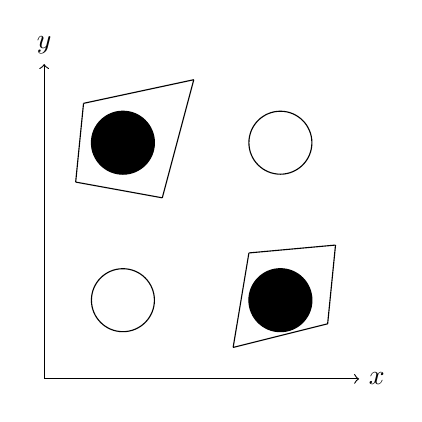
\begin{tikzpicture}
        
            \draw [fill=black] (0.5,1) circle [radius=0.4];
            \draw [] (0.5,-1) circle [radius=0.4];
    
            \draw [] (2.5,1) circle [radius=0.4];
            \draw [fill=black] (2.5,-1) circle [radius=0.4];
    
            \draw[-] (0, 1.5) -- (-0.1,0.5);
            \draw[-] (-0.1, 0.5) -- (1,0.3);
            \draw[-] (1, 0.3) -- (1.4,1.8);
            \draw[-] (1.4, 1.8) -- (0,1.5);
    
            \draw[-] (1.9, -1.6) -- (3.1, -1.3);
            \draw[-] (3.1, -1.3) -- (3.2,-0.3);
            \draw[-] (3.2, -0.3) -- (2.1,-0.4);
            \draw[-] (2.1, -0.4) -- (1.9,-1.6);
    
            
            \draw[->] (-0.5,-2) -- (3.5,-2) node[right] {$x$};
            \draw[->] (-0.5,-2) -- (-0.5, 2) node[above] {$y$};
        \end{tikzpicture}
        \caption{Using non-linear activation functions}% TODO denne kunne trenge mer forklaring
        % TODO verifiser formen på denne? den forrige har linje, men denne har ikke (?)
        % Denne er riktig tegnet, men klassifiseringen må fylles inn, og problemet må forklares bedre
        % Reagerte bare på at den første har linjer og denne ikke. http://www.ece.utep.edu/research/webfuzzy/docs/kk-thesis/kk-thesis-html/node19.html for eksempel.. Bare nysgjerrig

    \end{subfigure}
    
    \caption{Figure of the exclusive-OR problem, by the capabilities of a model with non-linear activation functions versus no activation function.}
    \label{fig:exclusive-OR problem}
\end{figure}

Activation functions are also important for squashing the output of a neural network into desired bounds. A common use case is to convert the network output to probabilities, where softmax is often used as the activation function for the last layer. Softmax is an activation function which transforms its inputs to a combined sum of 1 \cite{sharma_understanding_2018}.

\begin{figure}[H]
  \centering
    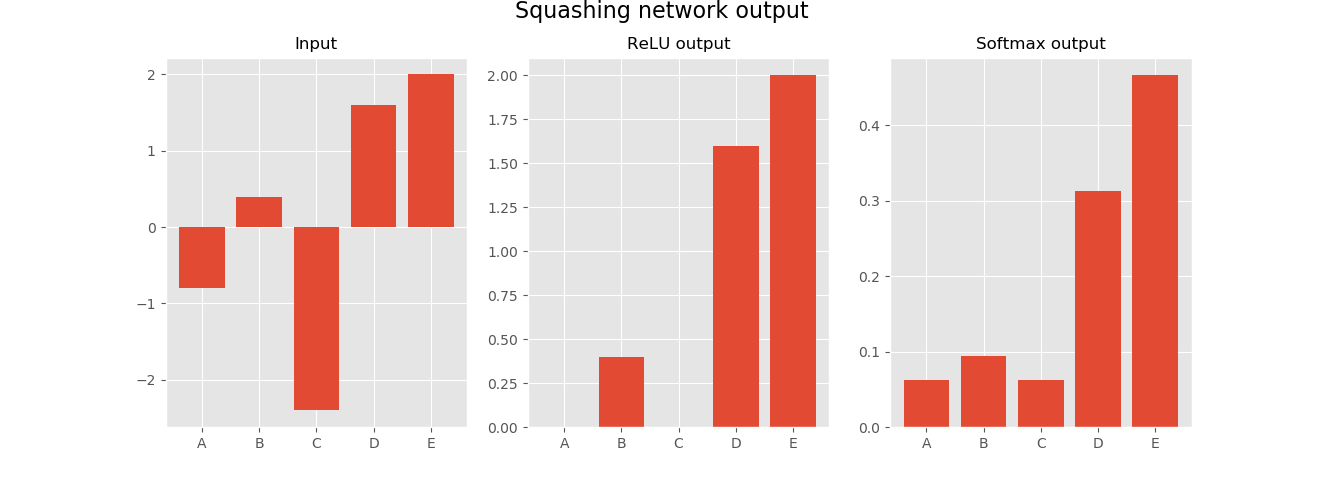
\includegraphics[width=\textwidth]{Assets/Chapter2_Theory/squashin_output_data_using_activation_functions.png}
    \caption{Figure of how example input data is transformed through two different activation functions. Data flows from left to right, with output from the previous graph used as input to the next.}
\end{figure}

\subsubsection{ReLU}

Rectified linear unit or ReLU is a nonlinearity introduced by Hanloser et al. in 2000 \cite{smith_scientist_1997}, and has later been found successful as a nonlinearity in deep neural network. This function disallows negative values, meaning that the output from all negative input values is 0. If the input value is positive, the same value is returned.

%It is a function which disallows negative values, and outputs the input if positive, else it outputs 0.

\begin{equation} \label{eqn:relu}
    f(x) = max(x, 0)
\end{equation}

% The max operation used in the ReLU activation function is calculated using the mathematical operations; addition, multiplication and comparison. These are cheap operations for a computer to perform, and ReLU is therefore a performant function. Especially compared to other activation functions who depend on calculating expensive exponential functions.
ReLU is a performant mathematical operation, as the $max$ operation only includes addition, multiplication and comparison, while other previously popular nonlinearities are dependent on calculating exponential functions. 

ReLU has also given good results compared to other nonlinearities in stochastic gradient descent (SGD). Krizhevsky et al. demonstrated an improvement of a factor of six, when comparing number of epochs needed to reach 25\% error rate with a network using ReLU, compared to an equivalent network with tanh as a nonlinearity \cite{krizhevsky_imagenet_2012}.

A negative side effect from ReLU is the dying ReLU problem, where neurons can be pushed to a state where the neuron will output the same value regardless of input. This is a variation of the vanishing gradient problem (\ref{vanishing-gradient}). The concept of dead neurons is described in \ref{dead-neurons}  \cite{zeiler_rectified_2013}.

\subsubsection{Softmax}

Softmax is an activation which transforms its inputs to a distribution with sum of one. This makes the softmax function useful to represent probabilities, and is therefore often used on the last layer of neural networks. Combined with the loss function categorical cross entropy (\ref{categorical-crossentropy}), softmax can be used to perform multiclass classification \cite{_cs231n_????-1}.
\begin{equation} \label{eqn:softmax}
    f_j(z) = \frac{e^{z_j}}{\sum_k e^{z_k}}
\end{equation}

\subsubsection{Sigmoid}

Sigmoid has been historically popular as an activation function in neural networks \cite{_neural_2018}. It works by squashing the input to the range $[0, 1]$, where small numbers are returned as a value close to 0, and large numbers are returned as values close to 1. 

\begin{equation} \label{eqn:sigmoid}
    \sigma(x) = \frac{1}{1 + e^{-x}}
\end{equation}

An issue with sigmoid is that the outputs are not zero-centered, which means the output of the function will all be of the same sign. When these values are sent to the next layer of the network, the inputs will cause the gradients to be the same sign as well. This can cause undesirable updates of weights during backpropagation, with zig-zag dynamics for weight updates \cite{_neural_2018}.

\subsubsection{Tanh}

Tanh is an activation function with similar characteristics as sigmoid, and can be represented as a scaled sigmoid (which can be seen in the equation below).

Tanh, however, squashes the inputs to the range $[-1, 1]$, which means it does not inherit the same issues with non zero-centered outputs. Therefore, in practice, tanh is always preferred to sigmoid \cite{_neural_2018}.

\begin{equation} \label{eqn:tanh}
    tanh(x) = 2 \cdot \sigma(2x) - 1 = \frac{2}{1+e^{-2x}} -1
\end{equation}

\subsection{Loss functions}
\label{loss_function}

Loss functions, also called error functions or cost functions, is used to calculate the margin between the expected value, and the predicted value in a neural network. These are used in conjunction with gradient descent, in order to update the weights and biases.

A commonly used loss function is mean squared error (MSE)
\begin{equation}
    \frac{1}{n} \sum^n_{i=1} (Y_i - \hat{Y_i})^2
\end{equation}

In MSE, the error is measured by finding the mean error (Expected value - Predicted Value) squared. By squaring the error, outliers are punished exponentially more than small errors. The error function can therefore be used to shape what the network should avoid, and what it should allow more of.%do more of.

\subsubsection{Crossentropy}
\label{categorical-crossentropy}

Crossentropy is a loss function typically used for classification tasks. Binary crossentropy is used when there are only two different classes, while categorical crossentropy is used for multiclass classification.

In order to represent the loss between a predicted class probability distribution and the correct distribution, we use a format called one-hot encoding. An example for predicting letters, we define three vectors; $C$ (classes), $\hat{Y}$ (truth) and $Y$ (prediction).


% https://www.youtube.com/watch?v=ErfnhcEV1O8
%https://rdipietro.github.io/friendly-intro-to-cross-entropy-loss/

\begin{equation} \label{eqn:catcross_ex1}
\begin{split}
    C &= [A, B, C, D] \\
    \hat{Y} &= [0.6, 0.1, 0.2, 0.1] \\
    Y &= [1.0, 0.0, 0.0, 0.0]
\end{split}
\end{equation}

Cross entropy can be calculated through the following equation.

\begin{equation} \label{eqn:catcross_ex2}
    H(Y, \hat{Y}) = \sum_i Y_i \log \frac{1}{\hat{Y}_i} = -\sum_i Y_i \log \hat{Y}_i
\end{equation}

Using the example from above. We calculate the error of prediction $\hat{Y}$ as.

\begin{equation} \label{eqn:catcross_ex3}
\begin{split}
    H(Y, \hat{Y}) = \\
    -( 1.0 \cdot \log 0.6\\
    + 0.0 \cdot \log 0.1\\
    + 0.0 \cdot \log 0.2\\
    + 0.0 \cdot \log 0.1) \\
    = - 1.0 \cdot \log 0.6 \approx -0.51
\end{split}
\end{equation}

The network's prediction on the correct answer A is the only number affecting the resulting error. Therefore, if the predicted probability is close to 0, the error will get very large, and when the predicted probability is close to 1, the error will get very small \cite{brownlee_how_2017}.

\subsection{Training neural networks}
\label{training_with_backpropagation}

Backpropagation is an algorithm used in the training of a neural network. The algorithm was introduced by Werbos et al. in 1974 \cite{werbos_beyond_1974}, however, it was not until in 1986, in \cite{rumelhart_learning_1986} by Rumelhart et al. that the importance of the algorithm was acknowledged \cite{_backpropagation_????-1}. This section will explain the algorithm without going into details for the underlying mathematics. 

The algorithm has two phases, the forward phase and the backward phase. In the forward phase the output from each layer is calculated as in section \ref{artificial_neural_networks}. The final output is then compared to a target output specified by the training sample. By comparing these values, an error can be calculated. This error is then sent backwards through the neural network.

\begin{figure}[H]
  \centering

    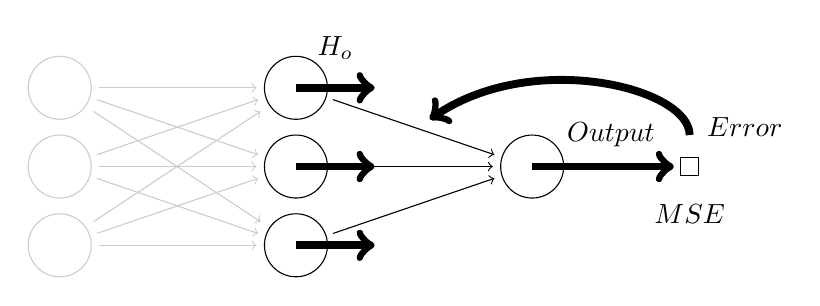
\begin{tikzpicture}
        
        \draw [draw={rgb:black,1;white,4}, ] (0.5,1) circle [radius=0.4];
        \draw [draw={rgb:black,1;white,4}, ] (0.5,0) circle [radius=0.4];
        \draw [draw={rgb:black,1;white,4}, ] (0.5,-1) circle [radius=0.4];

        \draw [] (3.5,1) circle [radius=0.4];
        \draw [] (3.5,0) circle [radius=0.4];
        \draw [] (3.5,-1) circle [radius=0.4];

        \draw [] (6.5, 0) circle [radius=0.4];

        \draw[draw={rgb:black,1;white,4}, ->] (1,1) -- (3,1);
        \draw[draw={rgb:black,1;white,4}, ->] (0.97,0.85) -- (3.02,0.15);
        \draw[draw={rgb:black,1;white,4}, ->] (0.93,0.7) -- (3.05,-0.7);

        \draw[draw={rgb:black,1;white,4}, ->] (0.97,0.15) -- (3.02,0.85);
        \draw[draw={rgb:black,1;white,4}, ->] (1,0) -- (3,0);
        \draw[draw={rgb:black,1;white,4}, ->] (0.97,-0.15) -- (3.02,-0.85);

        \draw[draw={rgb:black,1;white,4}, ->] (0.93,-0.7) -- (3.05,0.7);
        \draw[draw={rgb:black,1;white,4}, ->] (0.97,-0.85) -- (3.02,-0.15);
        \draw[draw={rgb:black,1;white,4}, ->] (1,-1) -- (3,-1);
        
        \draw[->] (3.97,0.85) -- (6.02,0.15);
        \draw[->] (4, 0) -- (6,0);
        \draw[->] (3.97, -0.85) -- (6.02,-0.15);
        
        \draw[->, line width=1mm] (3.5,1) -- (4.5,1);
        \draw[->, line width=1mm] (3.5,0) -- (4.5,0);
        \draw[->, line width=1mm] (3.5,-1) -- (4.5,-1);
        
        \draw[->, line width=1mm] (6.5,0) -- (8.3,0);
        
        \node at (7.5,0.4) {$Output$};
        \node at (4,1.5) {$H_o$};
        
        \node[draw] at (8.5,0) () {};
        \node at (8.5,-0.6) {$MSE$};
        \node at (9.2,0.5) {$Error$};
        
        \draw [->, line width=1mm] (8.5,0.4) .. controls (8.5,1) and (6.5,1.5) .. (5.2,0.6);
    \end{tikzpicture}
    \caption{Finding the error with mean squared error and sending it backwards.}
    \label{fig:backprop_one} 
\end{figure}

To actually train a neural network the weights between each layer has to be modified to reduce the overall error of the output. Gradient descent is used for this, where the partial derivatives for the error produced by a unit is calculated with respect to each of the connected weights.

For the neural network in figure \ref{fig:backprop_one}, the error from the output layer is first used to calculate the modifications for the weights between the hidden layer and the output layer. Then, the process is repeated for each of the hidden units. Three new errors is calculated, one for each of the hidden units. Finally, these errors are used to calculate the modifications for the weights between the input layer and hidden layer.

\begin{figure}[H]
  \centering

    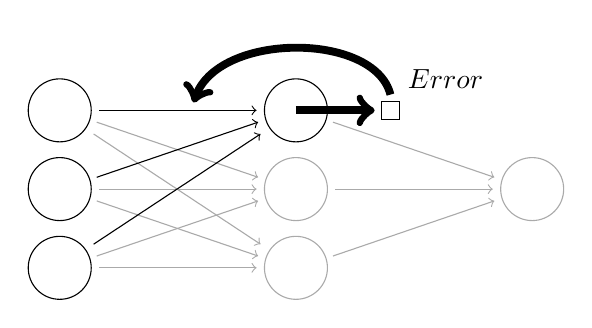
\begin{tikzpicture}
        
        \draw [] (0.5,1) circle [radius=0.4];
        \draw [] (0.5,0) circle [radius=0.4];
        \draw [] (0.5,-1) circle [radius=0.4];

        \draw [] (3.5,1) circle [radius=0.4];
        \draw [draw={rgb:black,2;white,4}, ] (3.5,0) circle [radius=0.4];
        \draw [draw={rgb:black,2;white,4}, ] (3.5,-1) circle [radius=0.4];

        \draw [draw={rgb:black,2;white,4}, ] (6.5, 0) circle [radius=0.4];

        \draw[->] (1,1) -- (3,1);
        \draw[draw={rgb:black,2;white,4}, ->] (0.97,0.85) -- (3.02,0.15);
        \draw[draw={rgb:black,2;white,4}, ->] (0.93,0.7) -- (3.05,-0.7);

        \draw[->] (0.97,0.15) -- (3.02,0.85);
        \draw[draw={rgb:black,2;white,4}, ->] (1,0) -- (3,0);
        \draw[draw={rgb:black,2;white,4}, ->] (0.97,-0.15) -- (3.02,-0.85);

        \draw[->] (0.93,-0.7) -- (3.05,0.7);
        \draw[draw={rgb:black,2;white,4}, ->] (0.97,-0.85) -- (3.02,-0.15);
        \draw[draw={rgb:black,2;white,4}, ->] (1,-1) -- (3,-1);
        
        \draw[draw={rgb:black,2;white,4}, ->] (3.97,0.85) -- (6.02,0.15);
        \draw[draw={rgb:black,2;white,4}, ->] (4, 0) -- (6,0);
        \draw[draw={rgb:black,2;white,4}, ->] (3.97, -0.85) -- (6.02,-0.15);
        
        \draw[->, line width=1mm] (3.5,1) -- (4.5,1);
        
        \node[draw] at (4.7,1) () {};
        \node at (5.4,1.4) {$Error$};
        \draw [->, line width=1mm] (4.7,1.2) .. controls (4.5,2) and (2.5,2) .. (2.2,1.1);


    \end{tikzpicture}
    \caption{Using error from the hidden units to calculate modification for the connected weights. The same process is repeated for the other hidden units.}
    \label{fig:backprop_two} 
\end{figure}


\subsection{Dropout}
\label{dropout}

Dropout is a technique used during training of a neural network. For a training sample, random units and all their connections are temporary dropped from the neural network \cite{srivastava_dropout:_2014}. This means that the connections dropped will not be updated for the current training sample. 

\begin{figure}[H]
\centering
    \begin{subfigure}{1\textwidth} 
    \centering
        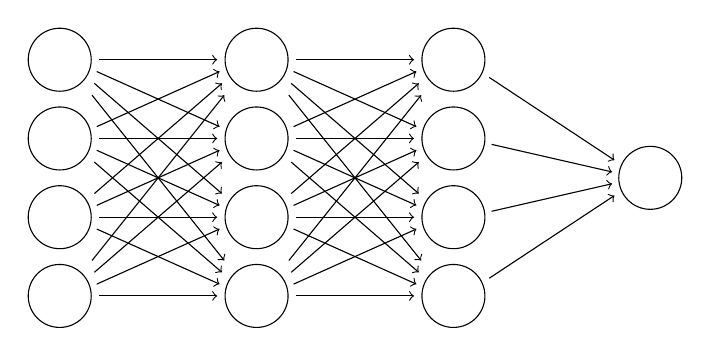
\begin{tikzpicture}

            \draw [] (-2.5,3) circle [radius=0.4];
            \draw [] (-2.5,2) circle [radius=0.4];
            \draw [] (-2.5,1) circle [radius=0.4];
            \draw [] (-2.5,0) circle [radius=0.4];

            \draw [] (0,3) circle [radius=0.4];
            \draw [] (0,2) circle [radius=0.4];
            \draw [] (0,1) circle [radius=0.4];
            \draw [] (0,0) circle [radius=0.4];

            \draw [] (2.5,3) circle [radius=0.4];
            \draw [] (2.5,2) circle [radius=0.4];
            \draw [] (2.5,1) circle [radius=0.4];
            \draw [] (2.5,0) circle [radius=0.4];
            
            \draw [] (5,1.5) circle [radius=0.4];
            
            
            \draw[->] (-2,3) -- (-0.5,3);
            \draw[->] (-2.03,2.85) -- (-0.47,2.15);
            \draw[->] (-2.06,2.7) -- (-0.44,1.30);
            \draw[->] (-2.09,2.55) -- (-0.41,0.45);
            
            \draw[->] (-2.03,2.15) -- (-0.47,2.85);
            \draw[->] (-2,2) -- (-0.5,2);
            \draw[->] (-2.03,1.85) -- (-0.47,1.15);
            \draw[->] (-2.06,1.70) -- (-0.44,0.30);
            
            \draw[->] (-2.06,1.3) -- (-0.44,2.7);
            \draw[->] (-2.03,1.15) -- (-0.47,1.85);
            \draw[->] (-2,1) -- (-0.5,1);
            \draw[->] (-2.03,0.85) -- (-0.47,0.15);
            
            \draw[->] (-2.09,0.45) -- (-0.41,2.55);
            \draw[->] (-2.06,0.30) -- (-0.44,1.7);
            \draw[->] (-2.03,0.15) -- (-0.47,0.85);
            \draw[->] (-2,0) -- (-0.5,0);
            
            
            \draw[->] (0.5,3) -- (2,3);
            \draw[->] (0.47,2.85) -- (2.03,2.15);
            \draw[->] (0.44,2.7) -- (2.06,1.30);
            \draw[->] (0.41,2.55) -- (2.09,0.45);
            
            \draw[->] (0.47,2.15) -- (2.03,2.85);
            \draw[->] (0.5,2) -- (2,2);
            \draw[->] (0.47,1.85) -- (2.03,1.15);
            \draw[->] (0.44,1.70) -- (2.06,0.30);
            
            \draw[->] (0.44,1.3) -- (2.06,2.7);
            \draw[->] (0.47,1.15) -- (2.03,1.85);
            \draw[->] (0.5,1) -- (2,1);
            \draw[->] (0.47,0.85) -- (2.03,0.15);
            
            \draw[->] (0.41,0.45) -- (2.09,2.55);
            \draw[->] (0.44,0.30) -- (2.06,1.7);
            \draw[->] (0.47,0.15) -- (2.03,0.85);
            \draw[->] (0.5,0) -- (2,0);
            
            
            \draw[->] (2.955,2.775) -- (4.545,1.725);
            \draw[->] (2.985,1.925) -- (4.515,1.575);
            \draw[->] (2.985,1.075) -- (4.515,1.425);
            \draw[->] (2.955,0.225) -- (4.545,1.275);
            
            
        \end{tikzpicture}
    \caption{}
    \label{fig:net_without_dropout}
    \end{subfigure}
    \begin{subfigure}{1\textwidth}
    \centering
        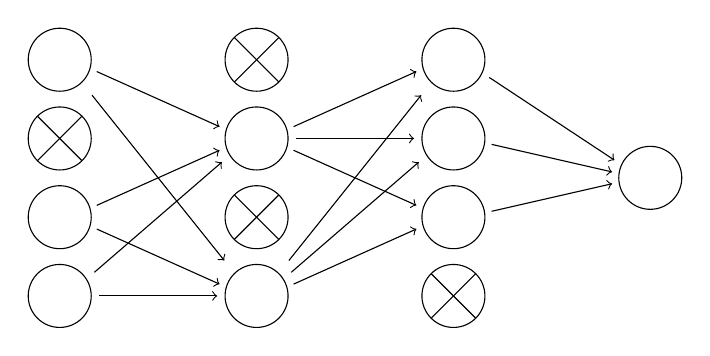
\begin{tikzpicture}
            \draw [] (-2.5,3) circle [radius=0.4];
            \draw [] (-2.5,2) circle [radius=0.4];
            \draw [] (-2.5,1) circle [radius=0.4];
            \draw [] (-2.5,0) circle [radius=0.4];

            \draw [] (0,3) circle [radius=0.4];
            \draw [] (0,2) circle [radius=0.4];
            \draw [] (0,1) circle [radius=0.4];
            \draw [] (0,0) circle [radius=0.4];

            \draw [] (2.5,3) circle [radius=0.4];
            \draw [] (2.5,2) circle [radius=0.4];
            \draw [] (2.5,1) circle [radius=0.4];
            \draw [] (2.5,0) circle [radius=0.4];
            
            \draw [] (5,1.5) circle [radius=0.4];
            
            \draw[-] (-2.78,2.28) -- (-2.22,1.72);
            \draw[-] (-2.78,1.72) -- (-2.22,2.28);
            
            \draw[-] (-0.28,3.28) -- (0.28,2.72);
            \draw[-] (-0.28,2.72) -- (0.28,3.28);
            
            \draw[-] (-0.28,1.28) -- (0.28,0.72);
            \draw[-] (-0.28,0.72) -- (0.28,1.28);
            
            \draw[-] (2.22,0.28) -- (2.78,-0.28);
            \draw[-] (2.22,-0.28) -- (2.78,0.28);
            
            
            \draw[->] (-2.03,2.85) -- (-0.47,2.15);
            \draw[->] (-2.09,2.55) -- (-0.41,0.45);
            
            \draw[->] (-2.03,1.15) -- (-0.47,1.85);
            \draw[->] (-2.03,0.85) -- (-0.47,0.15);
            
            \draw[->] (-2.06,0.30) -- (-0.44,1.7);
            \draw[->] (-2,0) -- (-0.5,0);
            
            
            \draw[->] (0.47,2.15) -- (2.03,2.85);
            \draw[->] (0.5,2) -- (2,2);
            \draw[->] (0.47,1.85) -- (2.03,1.15);
            
            \draw[->] (0.41,0.45) -- (2.09,2.55);
            \draw[->] (0.44,0.30) -- (2.06,1.7);
            \draw[->] (0.47,0.15) -- (2.03,0.85);
            

            \draw[->] (2.955,2.775) -- (4.545,1.725);
            \draw[->] (2.985,1.925) -- (4.515,1.575);
            \draw[->] (2.985,1.075) -- (4.515,1.425);
        \end{tikzpicture}
    \caption{}
    \label{fig:net_with_dropout}
    \end{subfigure}
\caption{Neural networks without (A) and with (B) dropout applied. The crossed circles are the dropped units.}
\label{fig:dropout_comparison}
\end{figure}

The purpose of dropout is to reduce the chance of overfitting a neural network. A neural network is overfitted when it is too closely related to the training samples, and not being as generalized as possible. An overfitted neural network will give good results if tested with the training data, but might fail on new data that the neural network has not seen before. Underfitting is the opposite of overfitting, and describes a too generalized network.

In a paper by Srivastava et al. from 2014 \cite{srivastava_dropout:_2014}, classifiers and neural networks trained with and without dropout applied is compared using standardized data sets. These data sets covers several areas, including vision, speech and text. In every comparison, neural networks with dropout was ranked high, if not highest.

\subsection{Common problems}
\label{vanishing-gradient}
\label{exploding-gradient}
\label{dead-neurons}
In artificial neural networks there are issues that optimization algorithms must overcome. The first issues to address is the vanishing and exploding gradient. These issues typically occur in deep feedforward- and recurrent networks (these types are described in the next sections). The common factor is that both types of artificial neural network generate long computational graphs. To explain this problem further, some mathematics is required.

A square matrix $A$ with $n$ linear eigenvectors $q_i (i=1..n)$ can be factorized as

\begin{equation} \label{eqn:mat_decomp}
    A=Q diag(\lambda) Q^{-1} 
\end{equation}

In equation \ref{eqn:mat_decomp} $A$ is our original matrix, $Q$ is an $nxn$ matrix where each column is an eigenvector $q_i$ and $diag(\lambda)$ is a diagonal matrix of eigenvalues. If we do this multiplication $t$ times, it only changes the number of times the diagonal matrix is multiplied \cite{weisstein_eigen_????}.

\begin{equation} \label{eqn:mat_decomp_t}
    A^{t} = Q diag(\lambda)^{t} Q^{-1}
\end{equation}

Both the vanishing and exploding gradient issues originate from the scaling according to the diagonal matrix with eigenvalues $diag(\lambda)$, with repeated multiplication by $A$. Vanishing gradient makes it difficult to find out in which direction parameters should move in order to move the cost function. While exploding gradients makes learning unstable \cite{goodfellow_deep_2016}.

Another issue with artificial neural networks is "dead" neurons (units), and is a direct cause of using ReLU. ReLU is widely used to not get caught in between gradient issues, however, it can cause weights to be updated in a way that makes the neuron unable to activate again \cite{_cs231n_????}.

\section{Feedforward neural networks}
% 
Feedforward neural networks, also referred to as deep feedforward networks or multilayer perceptrons (MLPs), are the most common deep learning models. The example network in figure \ref{fig:single_layered_neural_network} is a feedforward neural network. The ultimate goal of these networks is to approximate some function $f$, for example a task to classify (map) an input $x$ to a specific class $y$. In mathematical notation this can be written as $y = f(x)$. The networks mapping is defined as $y = f(x,\theta)$ where $\theta$ is learned in a way to approximate $f$ the best way. Goodfellow et al. \cite{goodfellow_deep_2016}[p.~163] explains why networks such as these are called feedforward.

\begin{displayquote}
\textit{These models are called feedforward because information flows through the function being evaluated from x, through the intermediate computations used to define f, and finally to the output y. There are no feedback connections in which outputs of the model are fed back into itself.}{\cite{goodfellow_deep_2016}[p.~163]}
\end{displayquote}

\subsection{Convolutional neural networks}

Convolutional networks \cite{lecun_generalization_1989} is also often referred to as convolutional neural networks or CNNs. CNNs are specialized for processing data that has a known typology. An example could be images, which is a 2D-grid of pixels. This project uses both images and sequential coordinates.

\begin{displayquote}
 \textit{Convolutional networks are simply neural networks that use convolution in place of general matrix multiplication in at least one of their layers.}{\cite{goodfellow_deep_2016}[p.~330]}
\end{displayquote}
To understand this further, the convolution operation needs to be explained. A convolution can be explained as an operation on two functions with real-valued arguments. 

% TRENGER VI EKSEMPEL? VELDIG LIKT GOODFELLOW
% TODO Trenger review; håv
Deep Learning by Goodfellow, Bengio and Courville explains a convolution with an example: we are tracking the location of a spaceship with a laser. Our laser is feeding us a single output x(t), which reads the position of the spaceship at time t. Now if the laser is noisy we may read data that could be unrepresentative. Thus, we could need some sort of average function. In addition, we would also like to specify that the most recent recordings are the most important ones. This is solvable using weights, where $w(a)$ is the weight function and $a$ is the age of a measurement \cite{goodfellow_deep_2016}.

\begin{figure}[H]
    \label{eqn:conv}
    \begin{equation}
    s(t) = \int x(a)w(t-a)da
    \end{equation}
    \caption{\cite{goodfellow_deep_2016}[p.~322] Example convolution which averages sensor readings and weights the most recent sensor readings. w(a) is the weighting function, x(t) is the position of the spaceship at time t. The result of this is a new function s, which gives us a smoothed estimate}
\end{figure}

\begin{figure}[H]
    \label{fig:conv_asterisk}
    \begin{equation}
        s(t) = (x*w)(t)
    \end{equation}
    \caption{Asterisk notation of a convolution.}
\end{figure}

% TRENGER VI EKSEMPEL? VELDIG LIKT GOOFELLOW
The first and second argument is often called the input and kernel, while the output is called the feature map. In the example with lasers $x$ would be our input and $w$ would be the kernel. % Eksempel på feature map ?
% Diskret notasjon
In a perfect world the laser would be able to provide real-time measurements, however, this is not realistic. Often readings are discretized, that means that a new reading will arrive at a given interval, an example of this could be a new reading every second. This would eventually lead to $t$ being an integer, and since both $x$ and $w$ is dependent on $t$ we end up with a discrete convolution \parencite{goodfellow_deep_2016}.

\begin{figure}[H]
    \label{fig:disc_conv}
    \begin{equation}
        s(t) = (x*w)(t) = \sum_{a=-\infty}^{\infty} x(a)w(t-a)
    \end{equation}
    \caption{Definition of the discrete convolution. \cite{goodfellow_deep_2016}[p.~323]}
\end{figure}

For two-dimensional inputs, two-dimensional kernels are used.

\begin{figure}[H]
    \label{fig:disc_conv2d}
    \begin{equation}
        S(i,j) = (I*K)(i,j) = \sum_{m} \sum_{n} I(m,n)K(i-m,j-n)
    \end{equation}
    \begin{equation}
        S(i,j) = (K*I)(i,j) = \sum_{m} \sum_{n} I(i-m,j-n)K(m,n)
    \end{equation}
    \caption{\cite{goodfellow_deep_2016}[p.~323] The two dimensional kernel in both it's original form in addition to the version with the flipped kernel. The last version is a result of flipping the kernel relative to it's input.}
\end{figure}

The actual function that usually exists in machine learning libraries is cross-correlation. Cross-correlation is the same as a convolution without flipping the kernel and is often referred as convolution.

\begin{figure}[H]
    \begin{equation}
        S(i,j) = (K*I)(i,j) = \sum_{m} \sum_{n} I(i+m,j+n)K(m,n)
    \end{equation}
    \label{fig:cross_corr}
    \caption{The cross-correlation function \cite{goodfellow_deep_2016}[p.~324].}
\end{figure}

Sparse interactions, connectivity or weights is a result of making the kernel smaller than the input. Even if an image has many thousands of pixels it is possible to extract small crucial features using smaller kernel sizes.

\begin{figure}[H]
    \centering
    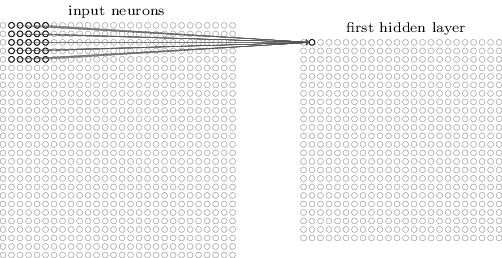
\includegraphics[width=\textwidth]{Assets/Chapter2_Theory/kernel_applied.png}
    \caption{\cite{nielsen_neural_2015} This figure shows how a convolution layer works with a 5x5 kernel, also referred to as a filter or feature detector. In this example, our input is 28x28, if we apply a 5x5 kernel we will end up with 24x24 units in the hidden layer. Available from http://neuralnetworksanddeeplearning.com/images/tikz45.png, 23.04.2018}
    \label{fig:kernel_applied}
\end{figure}

%In summary the convolutional layer accepts a volume of size $W_1$ x $H_1$ x $D_1$. In addition to a volume, it needs to provide four hyperparameters. These hyperparameters are the number of filters K, their spartial extent F, the stride S and the ammount of zero padding P. 
A convolutional layer has typically three stages, the first is to do the convolutions as illustrated in \ref{fig:kernel_applied}, these are linear activations. When all the convolutions are done, they are passed through a nonlinear activation function. An example of a nonlinear activation function is the sigmoid function from \ref{eqn:sigmoid}. Furthermore this stage is often referred to as the detector stage.

The last stage of the a typical convolutional layer is when we apply a pooling function to further modify the output \parencite{zhou_computation_1988}. A pooling function is able to replace the output of a small area with a summary of the nearby outputs. An example of a pooling function is the max pooling, which function uses a pooling unit with a specified size, for example 2x2. The pooling unit in a max pooling function simply outputs the maximum activation of it's region (2x2). A max pooling function with this pooling unit would turn 24x24 units to 12x12 units \cite{goodfellow_deep_2016} \cite{nielsen_neural_2015}.

\section{Recurrent neural networks}

Recurrent neural networks, also referred to as RNNs  are neural networks which can process sequential data \cite{rumelhart_learning_1986}. While CNNs are specialized on analyzing grid like data, such as images or videos, RNNs are more specialized on processing sequential data. The idea behind RNNs is to share parameters in different parts of a model. 

\begin{displayquote}
 \textit{Such sharing is particularly important when a specific piece of information can occur at multiple positions within the sequence.}{\cite{goodfellow_deep_2016}[p.~373]}
\end{displayquote}

Furthermore, an artificial neuron or computing unit is not only determined by it's activations in previous layers, it is now possible for an artificial neuron or computing unit to be determined by it's own activation earlier \cite{goodfellow_deep_2016} \cite{nielsen_neural_2015}.

\subsection{Long short-term memory}
\label{theory-LSTM}

Long short-term memory unit is a type of computational unit often used in recurrent neural networks. LSTM networks were introduces in 1997 by Sepp Hochreiter and Jürgen Schmidhuber \cite{hochreiter_long_1997}. LSTM networks has been improved in further research, for instance by giving the network the ability to forget \cite{gers_learning_1999}. These units can be utilized to keep important information over time, as opposed to traditional recurrent units, by adding new information on top of old state and not overriding it for each time step. This is described in a paper by J. Chung et al. \cite{chung_empirical_2014}.

\begin{displayquote}
    \textit{Intuitively, if the LSTM unit detects an important feature from an input sequence at early stage, it
    easily carries this information (the existence of the feature) over a long distance, hence, capturing
    potential long-distance dependencies.}{\cite{chung_empirical_2014}}
\end{displayquote}

LSTM layers typically consist of a several computational units. These will be referred to as \textit{memory cells}, and a collection of one or more cells will be referred to as \textit{memory blocks}. The input at the current timestep $t$ is notated with $x$, the output of the cells are notated by $h$, and the block's state is notated as $C$.

A key part of an LSTM memory block is the Constant Error Carousels (CEC) \cite{gers_learning_1999}, also known as state. This is visualized as the horizontal line in the top part of the figure below. The state flows through all cells in a memory block, and the state eventually determines the cell's output.

Each memory cell includes several gates, which are used to decide what the network should remember. These gates determine how the input should influence the state of the memory block. This is done through filters, which are combinations of a sigmoid activation function and a pointwise multiplication. These filters are known as gates. A typical LSTM memory cell has three gates, an input gate, output gate and a forget gate.

\begin{figure}[H]
    \centering
    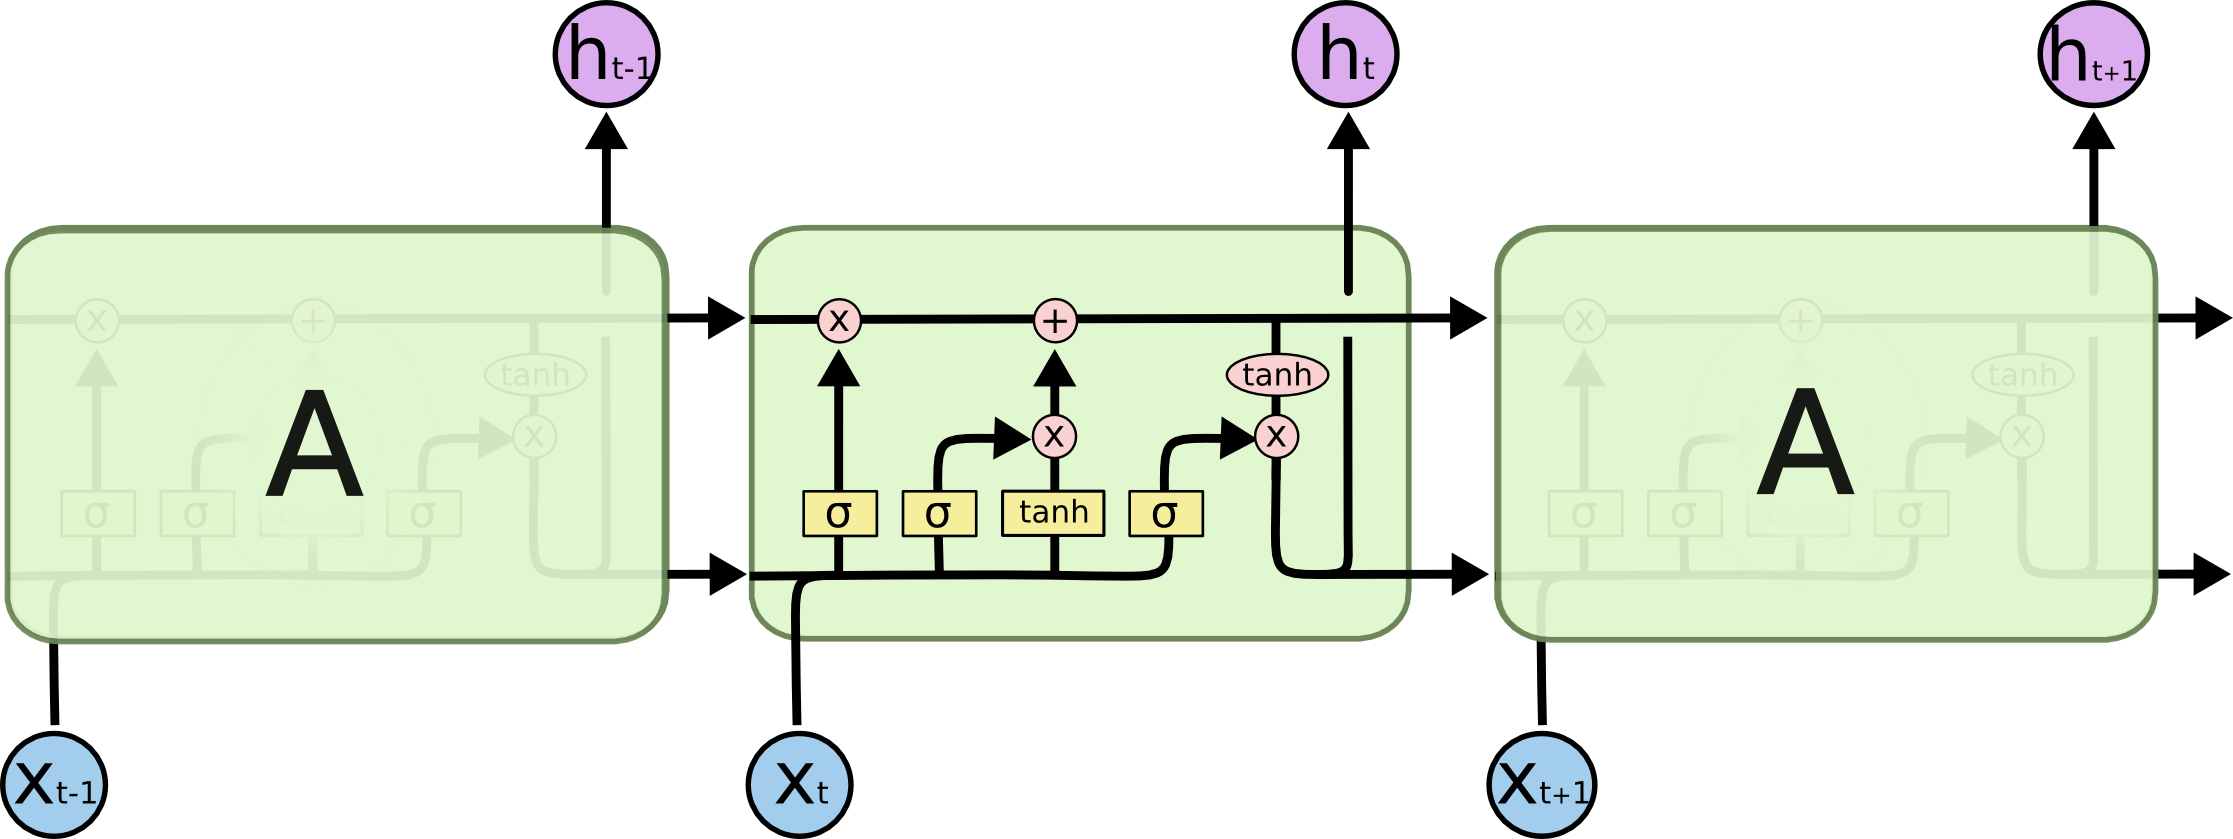
\includegraphics[width=\textwidth]{Assets/Chapter2_Theory/LSTM3-chain.png}
    \caption{Model of a memory block with three memory cells. The center cell includes a visualization of the different parts of the cell, and how the information flows inside the cell. The cell's input values are the current state of the memory block $C_{t-1}$ (top left), the output of the previous cell $h_{t-1}$ (bottom left), and  the current input value $x_t$. The upper line is the memory block's state, which flows through each cell of the block. The yellow squares are neural network layers with a specified activation function \cite{_understanding_2015}. Available from http://colah.github.io/posts/2015-08-Understanding-LSTMs/img/LSTM3-chain.png at 10-05-2018.}
    \label{fig:lstm_cells}
\end{figure}

The first gate in the memory cell is the input gate. This gate is notated as the combination of the sigmoid layer and the pointwise multiplication in the top left of the cell. This gate decides how much the previous cell's output $h_{t-1}$, and this timestep's input $x_t$ should influence the current state. The output of the sigmoid function is multiplied with the previous state $C_{t-1}$. If the output is 0, everything should be forgotten, and if the output is 1, everything should be remembered. 

The following layer with sigmoid activation determines how much of the current input should influence the memory state. This process is similar to the input gate. The layer noted by the $tanh$ activation function decides what should be remembered. The output of the pointwise multiplication between the sigmoid and tanh layer, is then added to the state.

The output of the memory cell is a filtered version of the current state, as seen top right in \ref{fig:lstm_cells}. The cell's state is run through a $tanh$ function, to squish the values in the range $[-1, 1]$, then the output is filtered through the output of the sigmoid function, similar to how state was removed and added in the previous steps. 

The sequential nature of these memory blocks makes LSTM networks good for predicting sequencial data. In pratice, most of the information we encounter is not needed for future predictions. By using gates, the LSTM network is able to decide which information should be remembered and to which scale the previously remembered information should influence future decisions \cite{gers_learning_1999} \cite{_understanding_2015}.

\subsection{Gated Recurrent Unit}

Gated Recurrent Unit is often referred to as GRU. It was recently proposed in 2014 by Cho et al. \cite{cho_learning_2014}, as an alternative to LSTM. GRU cells' advantage over LSTM is that it includes the same functionality in a less complex cell. This makes a GRU unit cheaper computationally, and has shown to outperform LSTM on models with fixed parameters \cite{chung_empirical_2014}. 

\begin{figure}[H]
    \centering
    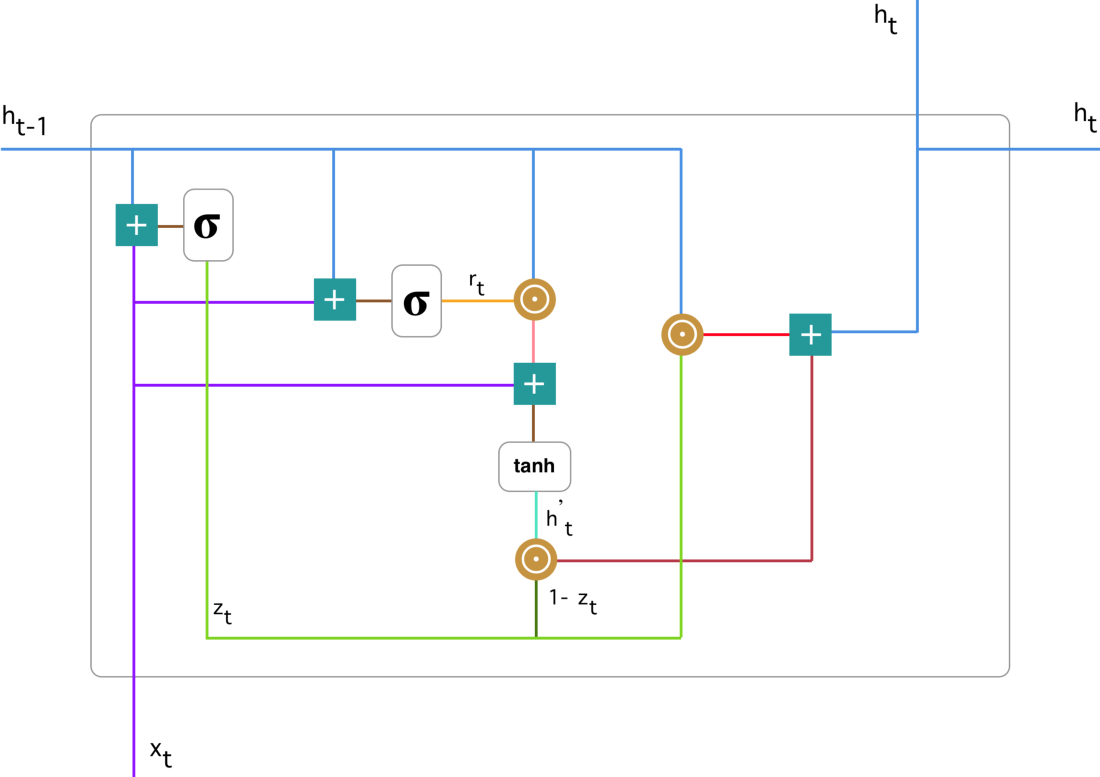
\includegraphics[width=\textwidth]{Assets/Chapter2_Theory/GRU-cell.png}
    \caption{A model of a Gated Recurrent Unit $h_{t-1}$ is the output of previous cell, $h_t$ is the output of current cell. $z_t$ is the output from the update gate. $r_t$ is the output of the reset gate. $x_t$ is the input at current timestep. Available at https://cdn-images-1.medium.com/max/800/1*6eNTqLzQ08AABo-STFNiBw.png (10-05-2018) \cite{kostadinov_understanding_2017}}.  
    \label{fig:gru-single-cell}
\end{figure}

The GRU cell calculates a temporary state from a combination of the previous state and the current input. The temporary state will be notated as $h_{tmp}$.

$h_{tmp}$ is calculated by adding the input at a timestep $x_t$ to a part of the previous state $h_{t-1}$. The influence of $h_{t-1}$ on $h_{tmp}$ is decided by the reset gate, $r_t$. This addition is then the input to a layer with a $tanh$ activation function, and results in $h_{tmp}$.

To calculate the output of the GRU cell, the cell needs to decide how much of the previous state it is going to keep. This is decided by the update gate $z_t$. Through a element-wise multiplication of $z_t$ with $h_{t-1}$, only the important parts of the previous state is kept. $h_{tmp}$ is multiplied element-wise with $1 - z_t$, and thereby the state removed from previous state is substituted with the state calculated in the current cell.

It is important to remember that the different gate's outputs is a value in the range $[0, 1]$, therefore if $z_t = 0$ then $1 - z_t = 1$

If the update gate is 0, $z_t = 0$, and none of the previous state should be kept. This leads to $1 - z_t = 1$, and the all the current state will be kept. On the other hand, if $z_t = 1$, the cell's output will equal the previous cell's output $h_{t-1} = h_t$, and the current input will not influence the output of the cell ($1 - z_t = 0$) \cite{kostadinov_understanding_2017}. 

\chapter{Technology and method}
\lhead{\emph{Technology and method}}

\section{Introduction}
% Var vi limited til å følge matistikk?
In this chapter the technology and methods applied in this project is reasoned. After reading this chapter, one should be able to get a basic understanding of the approach and be able to reconstruct the results. The nature of the assignment required us to use tools which delivers high productivity and flexibility. 

\section{Technology} % syns denne kan eksistere fint her
When collaboration tools were chosen the focus was on finding the best tool for the situation. Tools should handle rapid changes, collaboration tools needs a low response time and stability. % Share\LaTeX for document processing and collaboration, Slack for team communication and Office365 as a shared storage service. These tools combined with git and github make a powerful combination which easily could have been swapped with some other tool.  % er skrevet under

\subsection{Version control}
Throughout this project git has been used as version control. The nature of the project made us choose Github. Github was chosen on the basis of it's well established, stable and it enables remote collaboration.

%\subsection{Collaboration tools}
%When collaboration tools were chosen the focus was on finding the best tool for the situation. Tools should handle rapid changes, collaboration tools needs a low response time and stability. % Share\LaTeX for document processing and collaboration, Slack for team communication and Office365 as a shared storage service. These tools combined with git and github make a powerful combination which easily could have been swapped with some other tool.  % er skrevet under

%\subsubsection{Writing}
\subsection{Collaboration tools}
\LaTeX \ was chosen as document preparation system. \LaTeX \ makes it simpler to generate professional looking papers. It also has good support for writing equations, creating figures, and can be extended with packages to expand its functionality. ShareLaTeX was used for real time collaboration in the same \LaTeX \ document. 

For storage and mail Office365 was used (OneDrive and Outlook), this is a tool provided by NTNU for it's students. This platform enables us to easily communicate with our product owners and mentor in addition to storing our project documents and attachments.


\subsection{Python and frameworks}
The choice of programming language was influenced mainly by its ability to integrate into already existing techonlogy, and the availability of machine learning tools. Python was a natural choice as the current application (Matistikk), was written in Django. TensorFlow, a popular machine learning library written by Google, also has bindings to Python. For machine learning, Keras\cite{chollet_keras_2015}, which is a higher level machine learning library with integration to TensorFlow, was chosen. Keras has excellent documentation and it's functionality makes it a delight to use. Keras is well suited for quick prototyping and it provides the engineer with the productivity needed to make a proof of concept as quickly as possible.


A client application was also needed to draw symbols, collect data and present statistics. To keep the application architecture simple, regular HTML, CSS and JavaScript with JQuery was chosen. Tornado was chosen to serve the HTML file and the API. Tornado is a simple framework to build web servers in Python and  was chosen because of its simplicity and the availability of WebSockets.
% HTML file and 'an or the' API ???

\section{Architecture}
The data used in this project is both sequential coordinates from CROHME (InkML example: \ref{lst:InkML_ex}) and image data. Because our data was sequential it became natural to use a WebSocket in the initial development phase. Both to resemble data format and to build ideas around how to keep all the information which lies within sequential coordinates. 
For the sake of simplicity, it was also implemented a way to do this over a simple http post request as an alternative to the WebSocket implementation. Doing it this way created a simple, but solid foundation for the engineers behind Matistikk to do it the way they wanted. \\
%After discussion with our project owners, we were drawn to the direction of using a http post request. The test application also does not think about the amount of data it sends per classification request. If the canvas is changed, it still re-sends the entire buffer. This is both to easy re-evaluate the buffer, but in addition this can trigger changes in the segmentation process, which can eventually lead to a different classification. % tror ikke denne trengs

\section{Preparing data}
This section will go through the process from when each symbol was segmented, to how the symbols were converted to input in the neural networks.

The data used as train data for the neural networks was in an XML format called InkML. In order to use this data as input to the neural networks, two main preprocessing steps were made. The data was first parsed, converted to NumPy arrays and normalized, then converted to images.

The data received from the front end application was processed in the same way, however without parsing the InkML files. Opposed to the data received from InkML, this data was not already segmented, and this process had to be completed first. The process for segmenting symbols is described in \ref{the_recognintion_system}.

The motivation for converting data to images was to use already existing models created for the MNIST dataset as a fundation for further work.

\subsection{Traces}
The coordinates received from InkML and the front end application included coordinates at different scales. Therefore the traces had to be scaled, where the chosen scale was within the range $[-1, 1]$, while still keeping the same proportions. The scaling process is described in \ref{scale_linear_by_column}.

An example of a trace received from InkML can be seen in \ref{fig:sqrt_not_processed}.
\begin{figure}[H]
    \centering
    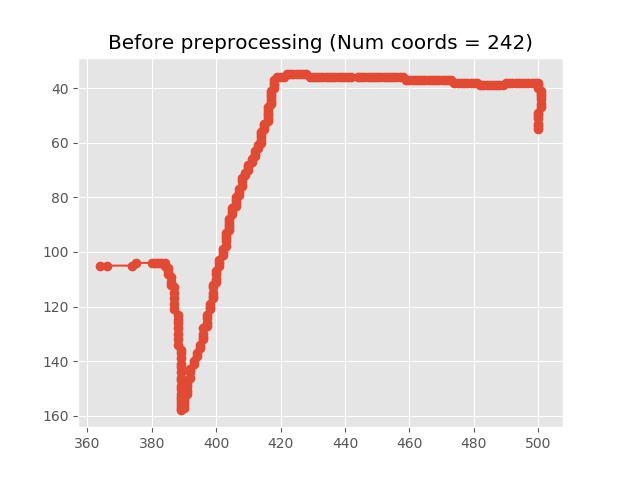
\includegraphics[width=\linewidth,keepaspectratio]{Assets/Chapter3_Method/sqrt_before_preprocessing.png}
    \caption{A square root which has not been through preprocessing.}
    \label{fig:sqrt_not_processed}
\end{figure}

The traces were recorded with different sampling frequencies. Some traces included several hundred points per symbol, while others included less than ten points per symbol. In order to improve performance of the networks, and make the input data normalized, the number of data points per symbol was reduced through a variant of the Ramer-Douglas-Peucker algorithm \ref{ramer_douglas_peucker}. All symbols' data points were reduced to a maximum of 40 data points. If the original tracing had less than 40 data points, it was padded using leading zeros. An example of the resulting trace which was used as input to the RNN model can be seen below.

\begin{figure}[H]
    \centering
    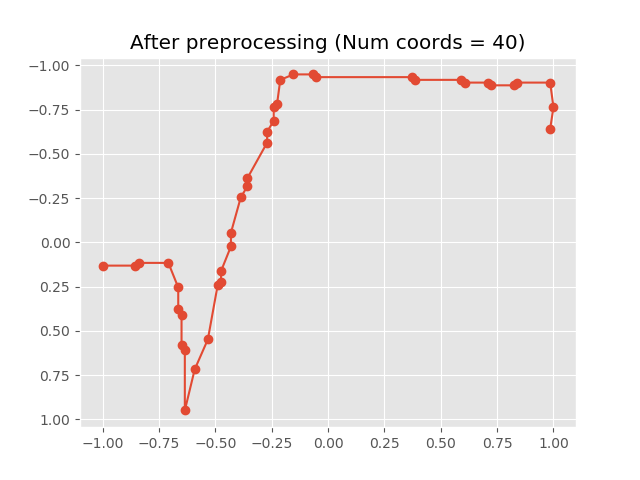
\includegraphics[width=\linewidth,keepaspectratio]{Assets/Chapter3_Method/sqrt_after_preprocessing.png}
    \caption{A square root after trace preprocessing.}
    \label{fig:sqrt_processed}
\end{figure}

\subsection{Images}

To prepare trace data for the convolutional neural network, the traces were converted into an image. In order to turn traces into images, the traces were first scaled by applying the the same scaling as previously \ref{scale_linear_by_column}, however within the range $[0, 26]$.

The next step was to generate an empty black image with 26x26 pixels (matrix of size 26x26 with only zeros). Afterwards, the pixels between each consecutive coordinate-pair were filled with white (255), and the resulting pixel grid was then normalized by dividing with 255. An example of the resulting grid presented as a matrix can be seen below, the example is simplified by using only a 8x10 matrix.

\begin{figure}[H]
    \begin{center}
    $
    \begin{bmatrix} % Jobbe mer forklaringen, vi scaler ikke 26x26 til 4x4 (?)
        \textcolor{gray}{0} & \textcolor{gray}{0} & \textcolor{gray}{0} & \textcolor{gray}{0} & \textcolor{gray}{0} & \textcolor{gray}{0} & \textcolor{gray}{0} & \textcolor{gray}{0} & \textcolor{gray}{0} & \textcolor{gray}{0} \\
        \textcolor{gray}{0} & \textcolor{gray}{0} & \textcolor{gray}{0} & \textcolor{gray}{0} & 1 & 1 & 1 & 1 & 1 & \textcolor{gray}{0} \\
        \textcolor{gray}{0} & \textcolor{gray}{0} & \textcolor{gray}{0} & 1 & \textcolor{gray}{0} & \textcolor{gray}{0} & \textcolor{gray}{0} & \textcolor{gray}{0} & \textcolor{gray}{0} & 1 \\
        1 & \textcolor{gray}{0} & \textcolor{gray}{0} & 1 & \textcolor{gray}{0} & \textcolor{gray}{0} & \textcolor{gray}{0} & \textcolor{gray}{0} & \textcolor{gray}{0} & \textcolor{gray}{0} \\
        \textcolor{gray}{0} & 1 & \textcolor{gray}{0} & 1 & \textcolor{gray}{0} & \textcolor{gray}{0} & \textcolor{gray}{0} & \textcolor{gray}{0} & \textcolor{gray}{0} & \textcolor{gray}{0} \\
        \textcolor{gray}{0} & 1 & \textcolor{gray}{0} & 1 & \textcolor{gray}{0} & \textcolor{gray}{0} & \textcolor{gray}{0} & \textcolor{gray}{0} & \textcolor{gray}{0} & \textcolor{gray}{0} \\
        \textcolor{gray}{0} & 1 & \textcolor{gray}{0} & 1 & \textcolor{gray}{0} & \textcolor{gray}{0} & \textcolor{gray}{0} & \textcolor{gray}{0} & \textcolor{gray}{0} & \textcolor{gray}{0} \\
        \textcolor{gray}{0} & \textcolor{gray}{0} & 1 & \textcolor{gray}{0} & \textcolor{gray}{0} & \textcolor{gray}{0} & \textcolor{gray}{0} & \textcolor{gray}{0} & \textcolor{gray}{0} & \textcolor{gray}{0} \\

    \end{bmatrix}
    $
    \end{center}
    \caption{An 8x10 matrix representing a pixel grid of a square root symbol.} % burde nok ha litt mer forklaring, TODO flytt forklaringen ovenfor ned i caption. (?)
    \label{fig:sqrt_matrix}
\end{figure}

\begin{figure}[H]
    \centering
    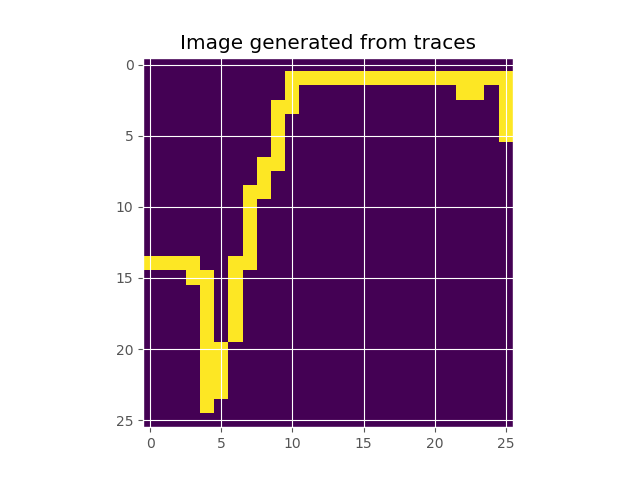
\includegraphics[width=\linewidth,keepaspectratio]{Assets/Chapter3_Method/sqrt_image.png}
    \caption{The resulting square root from the preprocessing done in previous steps.\\The generated image is 26x26 pixels.}
    \label{fig:sqrt_img}
\end{figure}

\section{The recognition system}
\label{the_recognintion_system}
The recognition system consists of both some "hard-coded" logic and the neural network. As stated in chapter \ref{handwriting_recognition}, handwriting recognition includes several steps required to classify correctly. The "hard-coded" logic solves the segmentation issue in an elementary way. The approach on the segmentation issue leaves the system vulnerable for noisy inputs. In addition, the system does a lot of preprocessing to make sure that the data flowing from the front end to the back end is roughly the same size, format, data type and so forth. 

[TODO] simple diagram of the whole process % vurder nødvendighet ?

\subsection{Preprocessing and segmentation}
%\section{Segmentation}
A large part of our approach relies on the segmentation of data, some symbols are put together by multiple traces, for example the number 4. Experimentation on finding the best solution for the segmentation issue led to object bounding boxes. Even though bounding boxes has potential to be the best solution for segmentation, it didn't perform as desired in terms of accuracy. In addition to it not proving to be as valuable as first thought we experienced good results with the previously mentioned "hard-coded" logic approach.

%The project went initially for a solution with a CNN, we had to separate the system into different tasks in order to make prediction. The reason behind this is that the CNN itself, in our solution should solely work on the classification of a symbol. Since our assignment is to handle symbols and expressions, we then need to extract single symbols from multiple symbols or expressions.\\
%This specific task was and is the most critical in order to get correct recognition with a CNN. If the segmentation turned out wrong, the classification would be handed bad data which makes a correct classification unlikely.\\ To solve the segmentation issue different approaches was attempted, among those were object localization and detection, with bounding boxes to easily detect symbols which consists of multiple strokes or traces. This idea of object detection was quite good and would have, if successful made the rest quite easy in comparison.\\ The attempts made on object detection was unsuccessful, we were getting results, but they were not proving to be better than solving it with a much simpler algorithm which did not require machine learning in the first place. 

[TODO] positional and proportional attributes assigned to the symbols


\subsection{Model architecture} % ?Classification | ?Models | ?Model architecture
Considering the lack of experience within the project participants, tutorials and articles needed to be read and understood. We quickly adapted and initially went after a solution with a CNN even though our primary data was sequential coordinates at that time. A recurrent network became more interesting after becoming more familiar with different use-cases and it's potential.

\textbf{TODO: Beskriv hva de ulike lagene er (dense = fully connected etc.)}

\subsubsection{RNN model}

The RNN model includes two one-dimensional convolution layers with max pooling and batch normalization. It also includes two bidirectional Gated Recurrent Unit layers. This model was first inspired by the Google Quick Draw model \cite{_recurrent_????}. It has been modified to correspond with the train dataset's input- and output data. The models architecture was also modified through experimentation to produce a better result on the test dataset.
\begin{figure}[H]
    \centering
    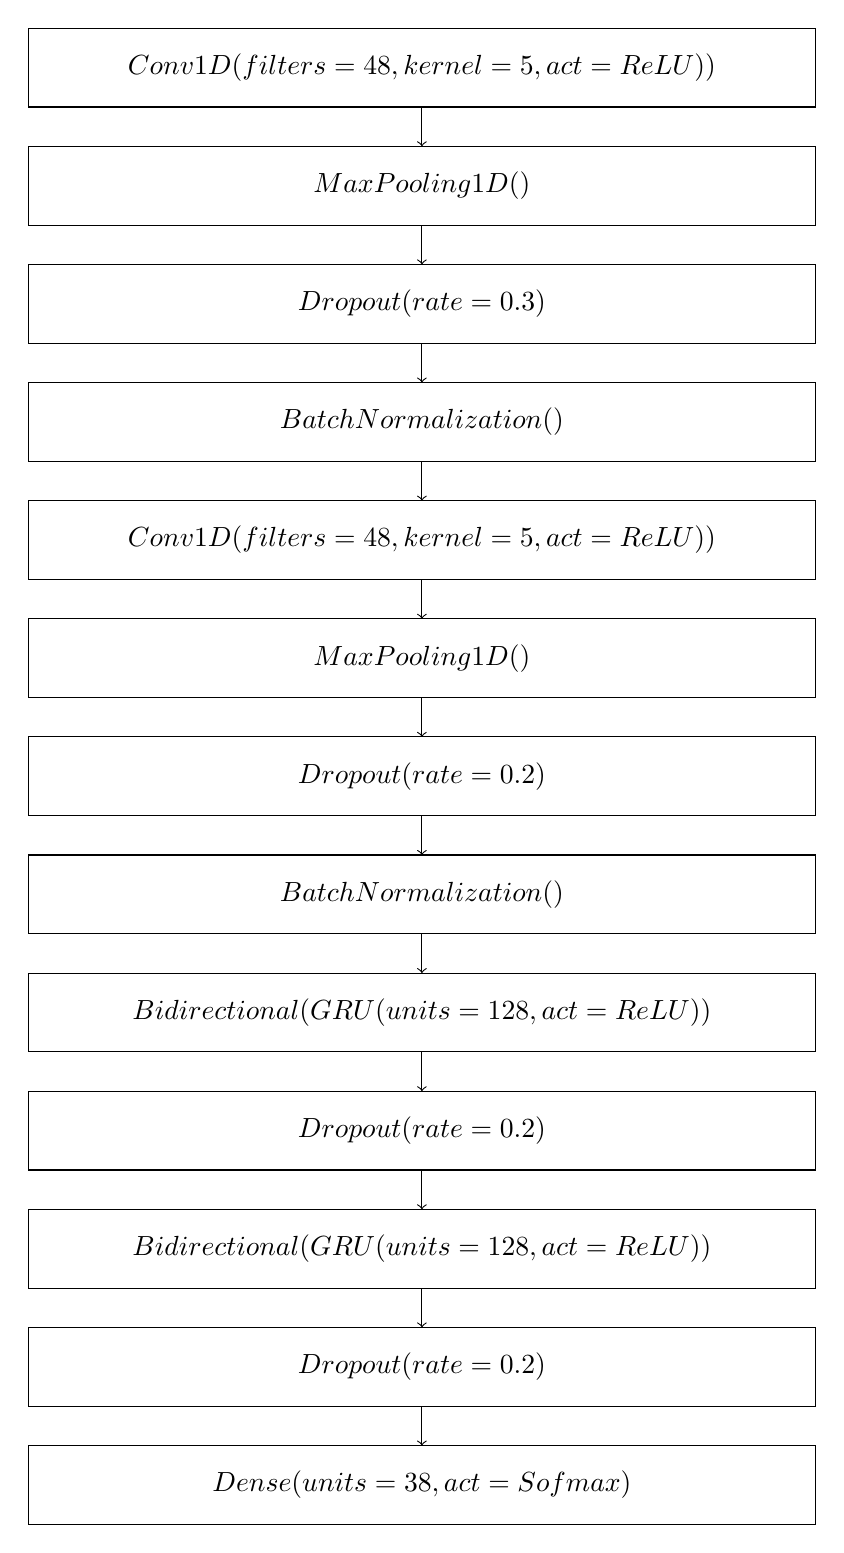
\begin{tikzpicture}
        \draw [black] (0, 1) rectangle (10, 0);
        \node[] at (5,0.5) {$Conv1D(filters=48, kernel=5, act=ReLU))$};
        \draw[->] (5, 0) -- (5, -0.5);
        
        \draw [black] (0, -0.5) rectangle (10, -1.5);
        \node[] at (5,0.-1) {$MaxPooling1D()$};
        \draw[->] (5, -1.5) -- (5, -2);

        \draw [black] (0, -2) rectangle (10, -3);
        \node[] at (5, -2.5) {$Dropout(rate=0.3)$};
        \draw[->] (5, -3) -- (5, -3.5);
        
        \draw [black] (0, -3.5) rectangle (10, -4.5);
        \node[] at (5, -4) {$BatchNormalization()$};
        \draw[->] (5, -4.5) -- (5, -5);
        
        \draw [black] (0, -5) rectangle (10, -6);
        \node[] at (5, -5.5) {$Conv1D(filters=48, kernel=5, act=ReLU))$};
        \draw[->] (5, -6) -- (5, -6.5);
        
        \draw [black] (0, -6.5) rectangle (10, -7.5);
        \node[] at (5, -7) {$MaxPooling1D()$};
        \draw[->] (5, -7.5) -- (5, -8);

        \draw [black] (0, -8) rectangle (10, -9);
        \node[] at (5, -8.5) {$Dropout(rate=0.2)$};
        \draw[->] (5, -9) -- (5, -9.5);
        
        \draw [black] (0, -9.5) rectangle (10, -10.5);
        \node[] at (5, -10) {$BatchNormalization()$};
        \draw[->] (5, -10.5) -- (5, -11);

        \draw [black] (0, -11) rectangle (10, -12);
        \node[] at (5, -11.5) {$Bidirectional(GRU(units=128, act=ReLU))$};
        \draw[->] (5, -12) -- (5, -12.5);

        \draw [black] (0, -12.5) rectangle (10, -13.5);
        \node[] at (5, -13) {$Dropout(rate=0.2)$};
        \draw[->] (5, -13.5) -- (5, -14);
        
        \draw [black] (0, -14) rectangle (10, -15);
        \node[] at (5, -14.5) {$Bidirectional(GRU(units=128, act=ReLU))$};
        \draw[->] (5, -15) -- (5, -15.5);
        
        \draw [black] (0, -15.5) rectangle (10, -16.5);
        \node[] at (5, -16) {$Dropout(rate=0.2)$};
        \draw[->] (5, -16.5) -- (5, -17);
        
        \draw [black] (0, -17) rectangle (10, -18);
        \node[] at (5, -17.5) {$Dense(units=38, act=Sofmax)$};


    \end{tikzpicture}
    \caption{A visualisation of the layer architecture in the RNN model.}
    \label{fig:RNN__model_visualization_1}
\end{figure}

\subsubsection{CNN model}

The CNN model has two convolution layers, a max pooling layer and two fully connected layers. The model had issues with overfitting, and it therefore includes two dropout layers with  rate of 25\% and 50\% respectively. The model also includes a flatten layer. The flatten layer performs a dimensionality reduction on the matrix returned from the convolutional layers. This model is inspired by CNN models with good results on the MNIST dataset. \textbf{TODO: Kilde for en paper med lignende arkitektur}
\begin{figure}[H]
    \centering
    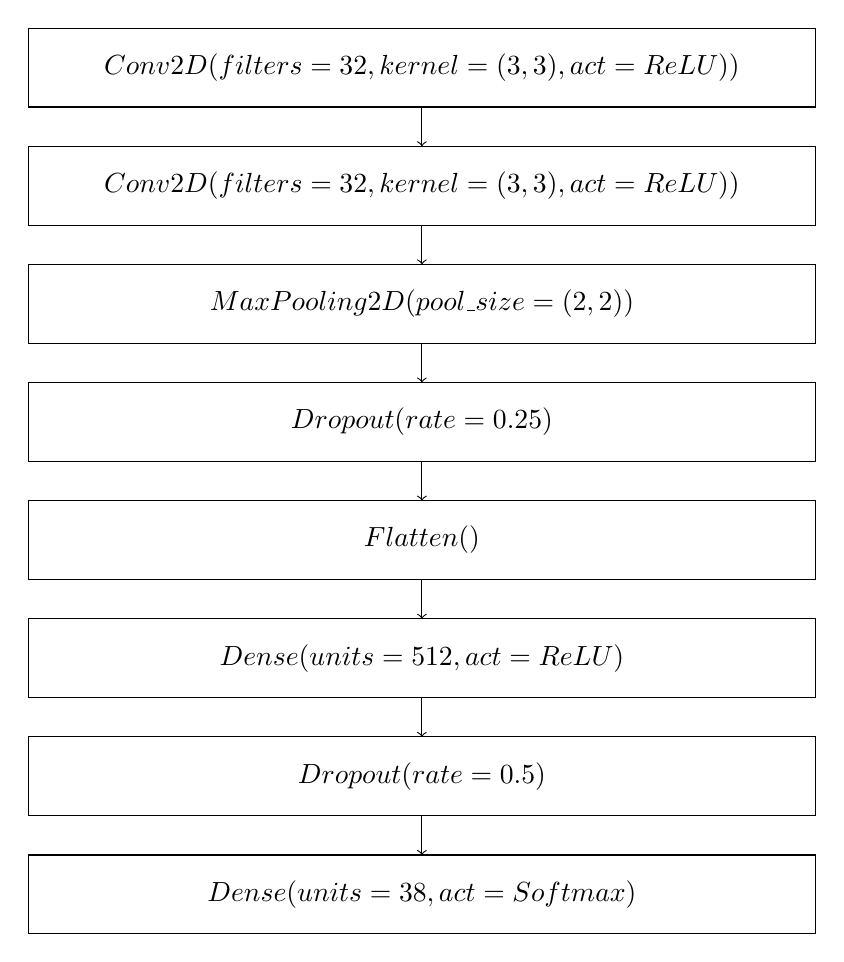
\begin{tikzpicture}
        \draw [black] (0, 1) rectangle (10, 0);
        \node[] at (5,0.5) {$Conv2D(filters=32, kernel=(3,3), act=ReLU))$};
        \draw[->] (5, 0) -- (5, -0.5);
        
        \draw [black] (0, -0.5) rectangle (10, -1.5);
        \node[] at (5,0.-1) {$Conv2D(filters=32, kernel=(3,3), act=ReLU))$};
        \draw[->] (5, -1.5) -- (5, -2);

        \draw [black] (0, -2) rectangle (10, -3);
        \node[] at (5, -2.5) {$MaxPooling2D(pool\_size=(2,2))$};
        \draw[->] (5, -3) -- (5, -3.5);
        
        \draw [black] (0, -3.5) rectangle (10, -4.5);
        \node[] at (5, -4) {$Dropout(rate=0.25)$};
        \draw[->] (5, -4.5) -- (5, -5);
        
        \draw [black] (0, -5) rectangle (10, -6);
        \node[] at (5, -5.5) {$Flatten()$};
        \draw[->] (5, -6) -- (5, -6.5);
        
        \draw [black] (0, -6.5) rectangle (10, -7.5);
        \node[] at (5, -7) {$Dense(units=512, act=ReLU)$};
        \draw[->] (5, -7.5) -- (5, -8);

        \draw [black] (0, -8) rectangle (10, -9);
        \node[] at (5, -8.5) {$Dropout(rate=0.5)$};
        \draw[->] (5, -9) -- (5, -9.5);
        
        \draw [black] (0, -9.5) rectangle (10, -10.5);
        \node[] at (5, -10) {$Dense(units=38, act=Softmax)$};

    \end{tikzpicture}
    \caption{A visualisation of the layer architecture in the CNN model.}
    \label{fig:RNN__model_visualization_2}
\end{figure}

\subsubsection{Combined model}

The combined model's architecture is a concatenation of the results from the CNN model, and the RNN model. The two models' last fully connected layer was removed before concatenation, to preserve as much information as possible. The combined model also has two fully connected layers and a dropout layer. The purpose of these layers is to enable the model to make its own predictions from the results of both input models.
\begin{figure}[H]
    \centering
    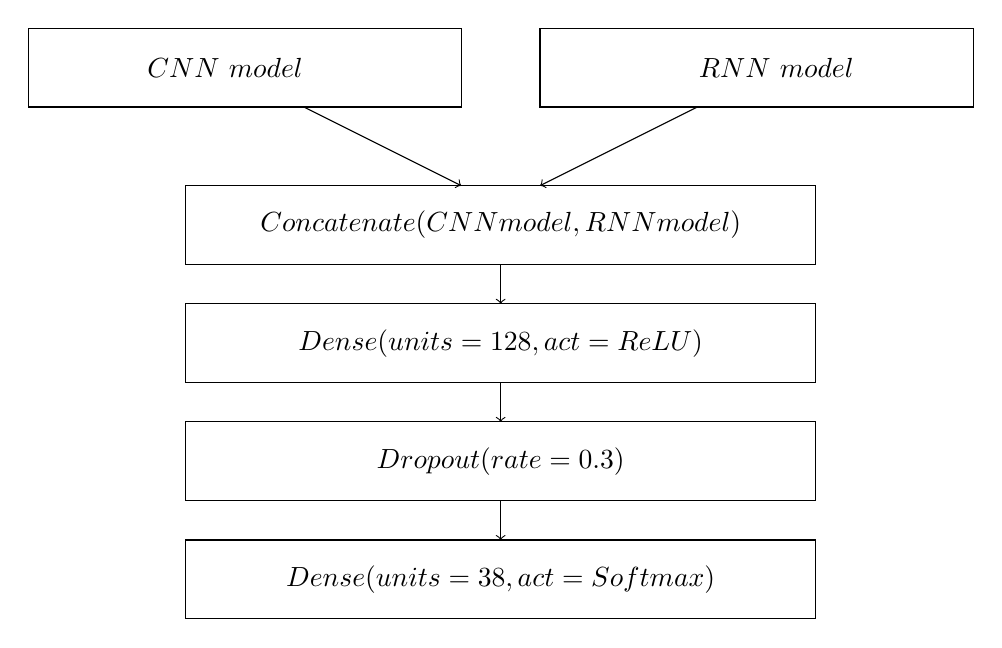
\begin{tikzpicture}
        \draw [black] (-6, -1) rectangle (-0.5, 0);
        \node[] at (-3.5,-0.5) {$CNN\ model$};
        \draw[[->] (-2.5, -1) -- (-0.5, -2);

        \draw [black] (0.5, -1) rectangle (6, 0);
        \node[] at (3.5,-0.5) {$RNN\ model$};
        \draw[[->] (2.5, -1) -- (0.5, -2);

        \draw [black] (-4, -2) rectangle (4, -3);
        \node[] at (0,-2.5) {$Concatenate(CNN model, RNN model)$};
        \draw[[->] (0, -3) -- (0, -3.5);
        
        \draw [black] (-4, -3.5) rectangle (4, -4.5);
        \node[] at (0,-4) {$Dense(units=128, act=ReLU)$};
        \draw[[->] (0, -4.5) -- (0, -5);
        
        \draw [black] (-4, -5) rectangle (4, -6);
        \node[] at (0,-5.5) {$Dropout(rate=0.3)$};
        \draw[[->] (0, -6) -- (0, -6.5);
        
        \draw [black] (-4, -6.5) rectangle (4, -7.5);
        \node[] at (0,-7) {$Dense(units=38, act=Softmax)$};

    \end{tikzpicture}
    \caption{A visualisation of the layer architecture in the combined model.}
    \label{fig:RNN__model_visualization_3}
\end{figure}
\subsection{Interpretation and context search}
%\section{Interpretation and context search} % SKRIVER LITT OM DETTE I \section{Segmentation}
% Har skrevet om at vi hardkodet segmentering, så ta det derfra. (fins i \section{Segmentation})

The interpretation system consist of a recursive search function and a set of fixed rules to determine the context of how the symbols fit together. This step receives a list of the classified symbols from the classification step as input and outputs the interpreted context in a tree based format of objects. This tree is sent back as a list of objects, where some of them links to other objects. % TODO review; er interpretation system rett ordbruk? 

\begin{figure}[H]
\begin{center}
    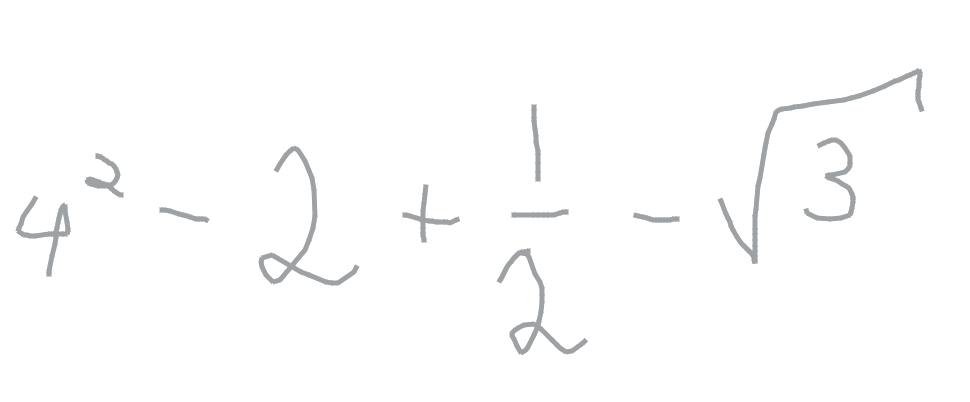
\includegraphics[scale=0.2]{Assets/Chapter3_Method/expression.png}
\end{center}
\centering
    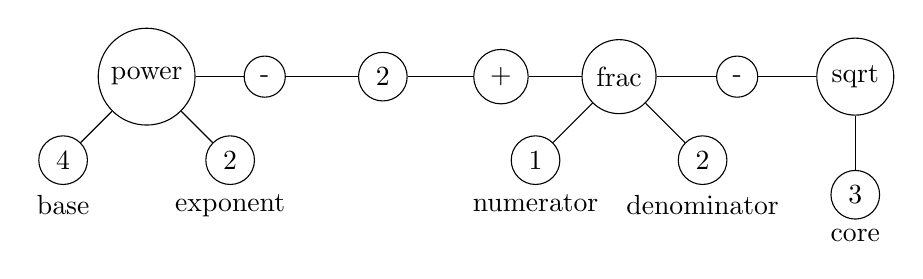
\begin{tikzpicture}[-,',auto,node distance=1.5cm,main node/.style={circle,draw}]
    \node[main node] (2) {power};
    \node[main node] (3) [right of=2] {-};
    \node[main node] (4) [right of=3] {2};
    \node[main node] (5) [right of=4] {+};
    \node[main node] (6) [right of=5] {frac};
    \node[main node] (7) [right of=6] {-};
    \node[main node] (8) [right of=7] {sqrt};
    
    \node[main node] (9) [below left of=2, label=below:base] {4};
    \node[main node] (10) [below right of=2, label=below:exponent] {2};
    
    \node[main node] (11) [below left of=6, label=below:numerator] {1};
    \node[main node] (12) [below right of=6, label=below:denominator] {2};
    
    \node[main node] (13) [below of=8, label=below:core] {3};
    
    

    \path[every node/.style={font=\sffamily\small}]
        (2) edge node [right] {} (3)
        (3) edge node [right] {} (4)
        (4) edge node [right] {} (5)
        (5) edge node [right] {} (6)
        (6) edge node [right] {} (7)
        (7) edge node [right] {} (8)
        (2) edge node [right] {} (9)
        (2) edge node [right] {} (10)
        (6) edge node [right] {} (11)
        (6) edge node [right] {} (12)
        (8) edge node [right] {} (13);

    \end{tikzpicture}
    \caption{An input expression and the resulting context tree.}

\label{fig:interpretation-tree1}
\end{figure}

% Dette kan kanskje legges i preprosessering et sted
%The symbols in the input list has a set of positional and proportional attributes that is used for sorting and to find all the symbols in an area. In addition, the attributes are used by the fixed rules to determine the notation used(see section frac-exp).


The system understands several mathematical notation elements, including square roots, fractions and exponents. Each of these elements has their own set of grammatical or positional rules that is used to find them (explained in section \ref{interpretation-square-roots} - \ref{interpretation-exponents}). In addition to these elements, some special symbols such as the equal sign and the multiplication dot is found and classified in this step (see section \ref{interpretation-special-symbols}).

\subsubsection{The main function}
% gangen i det hele
The main function in the interpretation system orchestrates the order of what element to search for. The order of elements searched for is:

\begin{enumerate}
    \setlength\itemsep{0.3em}
    \item Square roots
    \item Fractions
    \item Equal signs
    \item Multiplication dots
    \item Power groups, base and exponent
\end{enumerate}

The recursive part of this system comes from the square roots, fraction and exponents. If the body of a square root contains more than one symbol or object, the whole group is sent recursively to the main function. The same applies for the numerator and denominator found in fractions and for exponent-groups. The reason for this is to further search for context in these subgroups. For instance, fractions can have fractions as their numerator and exponents can consist of smaller expressions. 

This search process can be illustrated by a flowchart:

\begin{figure}[H]
\centering
    \begin{tikzpicture}[->,',auto,node distance=1.5cm,main node/.style={circle,draw},sub node/.style={draw}]
    \node[main node] (1) [label=above:Input] {};
    \node[sub node] (2) [below of=1] {Sqrt};
    \node[sub node] (3) [below of=2] {Frac};
    \node[sub node] (4) [below of=3] {$=$};
    \node[sub node] (5) [below of=4] {$\cdot$};
    \node[sub node] (6) [below of=5] {power};
    \node[main node] (7) [below of=6,label=below:Output] {};

    \path[every node/.style={font=\sffamily\small}]
        (1) edge node [right] {} (2)
        (2) edge node [right] {} (3)
        (3) edge node [right] {} (4)
        (4) edge node [right] {} (5)
        (5) edge node [right] {} (6)
        (6) edge node [right] {} (7)
        
        (2) edge[bend right=80] node [left] {core} (1)
        (3) edge[bend left=90] node [left] {numerator/denominator} (1)
        (6) edge[bend right=90] node [left] {exponent} (1);

    \end{tikzpicture}
    \caption{Flowchart of the order and recursion.}

\label{fig:interpretation_flowchart}
\end{figure}

To find the contents of a body (numerators, denominators, square roots), the interpretation system uses the positional values of the input symbols to check whether they are inside the bounds of an area or not. If their middle point is inside this area, they are added to the output group of the area search. This area is limited by a set of maximum and minimum x- and y-coordinates. These limits comes from a set of parameters required by the main function and the positional values of control units (square roots, fraction bars).

If a square root-, fraction- or exponent-element is found, the system creates an object of the correct type and links the relevant symbols to it. When creating one of these objects the traces for each of the input symbols are combined and new positional and proportional attributes are found.

Details about how these elements are found is described in the next sections.

\subsubsection{Square roots}
\label{interpretation-square-roots}
% detaljer om kvadratrot

The square root symbols are found by creating a list of all the input symbols classified as a square root sign, by filtering out all others. These are then sorted by width to make sure that the recursive logic is maintained when searching for the bodies. The widest one is most likely the outermost one if there are roots within roots. To find the bodies the system searches for objects within the bounds specified by the positional attributes of a square root. The widest square root is evaluated first.

\begin{figure}[H]
\centering
    \begin{tikzpicture}
        \node[anchor=south west,inner sep=0, scale=0.5] at (0,0) {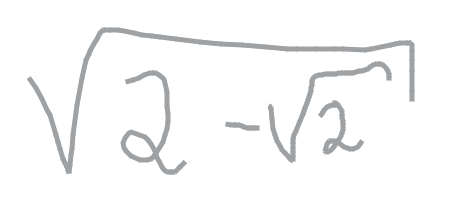
\includegraphics[width=\textwidth]{Assets/Chapter3_Method/interpretation-sqrt.png}};
        \draw[red, thick] (1.2,0.6) rectangle (6.7,2.8);
        \draw[blue, thick] (4.7,0.8) rectangle (6.3,2.3);
    \end{tikzpicture}
    \label{fig:interpretation}
\caption{Search area of square roots.}
\end{figure}

All the symbols and objects found inside are linked to the square root object as the body. This body is then sent recursively through the main function to find the context within the square root.

\begin{figure}[H]
\begin{center}
    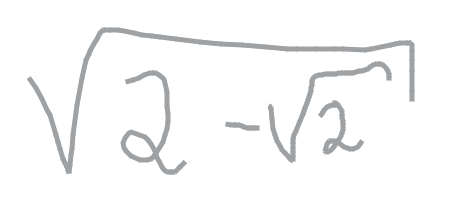
\includegraphics[scale=0.5]{Assets/Chapter3_Method/interpretation-sqrt.png}
\end{center}
\centering
    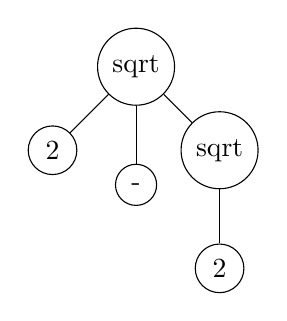
\begin{tikzpicture}[-,',auto,node distance=1.5cm,main node/.style={circle,draw}]
    \node[main node] (1) {sqrt};
    \node[main node] (2) [below left of=1] {2};
    \node[main node] (3) [below of=1] {-};
    \node[main node] (4) [below right of=1] {sqrt};
    \node[main node] (5) [below of=4] {2};

    \path[every node/.style={font=\sffamily\small}]
        (1) edge node [right] {} (2)
        (1) edge node [right] {} (3)
        (1) edge node [right] {} (4)
        (4) edge node [right] {} (5);

    \end{tikzpicture}
    \caption{An expression with a square root inside a square root and the resulting context tree.}

\label{fig:segmentation}
\end{figure}

\subsubsection{Fractions}

To find fractions the system searches for fraction bars by running the input symbols classified as minus signs through a test. To be classified as a fraction bar a minus sign must comply with one of the following cases:

\begin{itemize}
    \setlength\itemsep{0em}
    \item Have at least one symbol in the area over and under itself.
    \item Have at least two symbols in either the area over or the area under itself.
    \item Be the only minus sign in the input list and have at least one symbol in the area over or under itself.
\end{itemize}

To find the numerator and denominator of a fraction, the system searches for symbols in the area over and under the minus signs. The width of this area is specified by the leftmost and rightmost coordinate of the minus sign. The area never crosses the minus sign tested. The denominators and numerators found is also sent recursively through the main function to further look for context.

\begin{figure}[H]
\centering
\begin{tikzpicture}[-,',auto,node distance=1.5cm,main node/.style={circle,draw}]
    \node[anchor=south west,inner sep=0] (image) at (0,0) {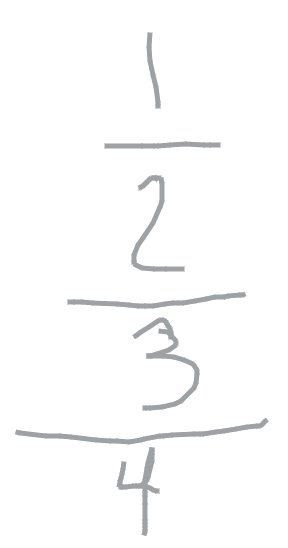
\includegraphics[width=0.2\textwidth]{Assets/Chapter3_Method/interpretation-frac.png}};
    
    \draw[red, thick] (0.2,0) rectangle (2.7,1.1);
    \draw[red, thick] (0.2,1.3) rectangle (2.7,6);
    \draw[blue, thick] (0.7,1.2) rectangle (2.5,2.5);
    \draw[blue, thick] (0.7,2.6) rectangle (2.5,6);
    \draw[purple, thick] (1.1,2.55) rectangle (2.2,4.1);
    \draw[purple, thick] (1.1,4.15) rectangle (2.2,6);
    
    \node [main node] (1) [right of=image, xshift=4cm, yshift=2cm]{frac};
    \node [main node] (2) [below left of=1]{frac};
    \node [main node] (3) [below right of=1]{4};
    \node [main node] (4) [below left of=2]{frac};
    \node [main node] (5) [below right of=2]{3};
    \node [main node] (6) [below left of=4]{1};
    \node [main node] (7) [below right of=4]{2};
    
    \node[rotate=45] (8) [below right of=5, xshift=-1cm, yshift=0.3cm]{denominators};
    \node[rotate=45] (9) [left of=2, xshift=0.5cm, yshift=1cm]{numerators};
    
    \path[every node/.style={font=\sffamily\small}]
        (1) edge node [right] {} (2)
        (1) edge node [right] {} (3)
        (2) edge node [right] {} (4)
        (2) edge node [right] {} (5)
        (4) edge node [right] {} (6)
        (4) edge node [right] {} (7);
\end{tikzpicture}
\caption{The search areas of a fraction expression with recursion and the corresponding context tree. The widest minus sign is considered the root fraction.}
\end{figure}

\subsubsection{Exponents}
\label{interpretation-exponents}

Exponents are found by checking if a pair of following symbols or objects forms a power-group. A power group is the object used for base/exponent groups. To form one of these groups the exponent has to be positioned such that the following rules are complied with:
\begin{itemize}
    \setlength\itemsep{0em}
    \item The lowest point of the exponent has to be higher up than the middle y-value of the base.
    \item The middle y value of the exponent has to higher up than the upper fourth of the base.
\end{itemize}
In addition, there is a special case rule if the exponent is an operator (-, +). Then, the lowest point of the exponent has to be higher up than the upper fourth of the base. The purpose of this is to increase the treshold to let a minus sign be the beginning of an exponent. Without this rule, expressions like '$2-2$' might mistakenly be recognized as '$2^{-}2$', since a minus sign is flat.

\begin{figure}[H]
\centering
\begin{tikzpicture}[-,',auto,node distance=1.5cm,main node/.style={circle,draw}]
    \node[anchor=south west,inner sep=0] (image) at (0,0) {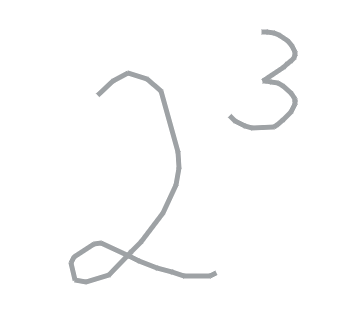
\includegraphics[width=0.2\textwidth]{Assets/Chapter3_Method/interpretation-exp.png}};
    \node[anchor=south west,inner sep=0] (image2) [left of=image, xshift=6cm] {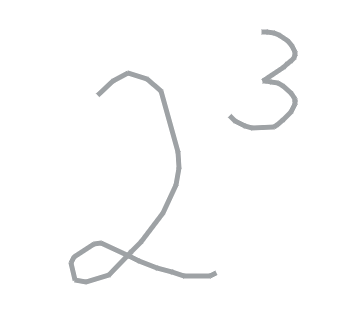
\includegraphics[width=0.2\textwidth]{Assets/Chapter3_Method/interpretation-exp.png}};
    
    \draw[-, red] (0,1.3) -- node[left, xshift=-2cm, yshift=-0.1cm] {middle point of base} (4,1.3);
    \draw[-, red] (0,1.65) -- node[left, xshift=-2cm, yshift=0.1cm] {lowest point of exp} (4,1.65);
    \draw[-, blue] (5,2.05) -- node[right, xshift=1.5cm, yshift=0.1cm] {middle point of exp} (8,2.05);
    \draw[-, blue] (5,1.7) -- node[right, xshift=1.5cm, yshift=-0.1cm] {top fourth of base} (8,1.7);
\end{tikzpicture}
\caption{Example of a power group and visualization of the first and second rule.}
\end{figure}

The system also supports groups of symbols and objects as base or exponent. Exponents within exponents is also supported. When a base and exponent is found, the system continues to check if the next symbol also is an exponent for the same base. This search continues until a symbol conflicts with one of the rules. All the found symbols is then sent recursively through the main function again.

\begin{figure}[H]
    \centering
    \begin{tikzpicture}[-,',auto,node distance=1.5cm,main node/.style={circle,draw}]
        \node[anchor=south west,inner sep=0] (image) at (0,0) {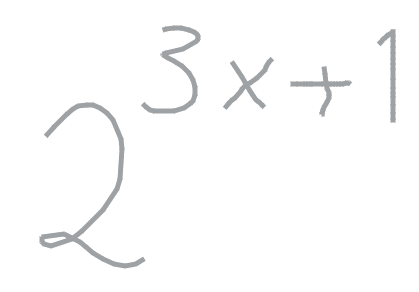
\includegraphics[width=0.2\textwidth]{Assets/Chapter3_Method/interpretation-exp2.png}};
    
        \node[anchor=south west,inner sep=0] (image2) [right of=image, xshift=4cm] {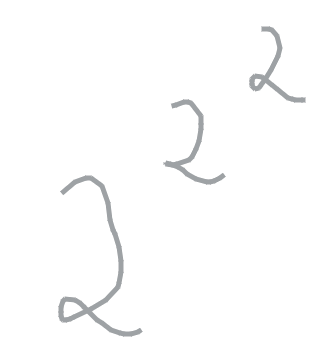
\includegraphics[width=0.2\textwidth]{Assets/Chapter3_Method/interpretation-exp3.png}};
        
        \node [main node] (1) [below of=image, yshift=-1.5cm]{power};
        \node [main node] (2) [below left of=1]{2};
        \node [main node] (3) [below right of=1]{group};
        \node [main node] (4) [below left of=3]{3};
        \node [main node] (5) [below of=3, xshift=-0.4cm]{x};
        \node [main node] (6) [below of=3, xshift=0.4cm]{+};
        \node [main node] (7) [below right of=3]{1};
        
        \node[rotate=0] (13) [left of=1, xshift=-0.2cm, yshift=-0.4cm]{Base};
        \node[rotate=0] (14) [right of=1, xshift=1cm, yshift=-0.4cm]{Exponent};
        
        \node [main node] (8) [below of=image2, yshift=-1.5cm]{power};
        \node [main node] (9) [below left of=8]{2};
        \node [main node] (10) [below right of=8]{power};
        \node [main node] (11) [below left of=10]{2};
        \node [main node] (12) [below right of=10]{2};
        
        \node[rotate=0] (15) [left of=11, xshift=0.5cm, yshift=0.4cm]{Bases};
        \node [] (16) [right of=10, xshift=0.4cm, yshift=-0.2cm]{Exponents};

        \path[every node/.style={font=\sffamily\small}]
            (1) edge node [right] {} (2)
            (1) edge node [right] {} (3)
            (3) edge node [right] {} (4)
            (3) edge node [right] {} (5)
            (3) edge node [right] {} (6)
            (3) edge node [right] {} (7)
            (8) edge node [right] {} (9)
            (8) edge node [right] {} (10)
            (10) edge node [right] {} (11)
            (10) edge node [right] {} (12);
            
    \end{tikzpicture}
    \caption{Power groups and their corresponding context tree.}
\end{figure}


\subsubsection{Special case symbols}
\label{interpretation-special-symbols}

In this system there are two special case symbols: the equal sign and the multiplication dot operator. These require special treatment due to how the segmentation and classification is done. An equal sign usually consist of two traces which would be interpreted as two minus signs since the segmentation step splits them up. The multiplication sign is a small dot that, when preprocessed and scaled up, would look similar to other round symbols like 0 and $\theta$. It would therefore most likely be misclassified.

To find equal signs the system searches for minus signs that are of similar size and lined up like an equal sign. To do this, each possible pair of minus signs in the input list is tested against some rules. The pair is classified as an equal sign only if these points are fulfilled:

\begin{itemize}
    \setlength\itemsep{0em}
    \item The width of the minus signs has to be similar. The difference in width has to be less than their average width.
    \item The difference between the center x-coordinate value has to be less than a third of their combined width.
    \item The difference between the center y-coordinate value has to be less than a their average width.
\end{itemize}

These rules became such after many rounds of testing. The idea behind them was to be as general as possible.

To find the multiplication signs the system searches for small symbols by looking at width, height and area. Symbols are classified as multiplication signs if these rules are fulfilled:

\begin{itemize}
    \setlength\itemsep{0em}
    \item The area (height*width) of the symbol has to be less than 250.
    \item Both the height and width has to be less than 20.
    \item The height and width has to be similar. One of them cannot be more than twice the other.
\end{itemize}

\subsection{Converting to \LaTeX}
After the context has been found, the results can be converted to the corresponding \LaTeX -code. For this, the truth values to all the output objects is combined in a string by a function. This function also has to be recursive, since the output objects might be fractions, square root or base-exponent groups. If a fraction is found, the contents of the numerator and denominator is sent through the same function. The same applies for the square root cores, exponents and bases.

\section{The project process} % 
The project process in terms of software engineering methodology had been a mix between multiple concepts and paradigms. Methodologies from the agile world were mostly used, such as tri programming. In the early stages of the project, we followed to some extent a methodology called Lean startup. Lean startup focuses on creating a minimal viable product, often referred to as \gls{MVP}. When the MVP was out, constructive discussions with the product owners about what they liked and what they did not like. At a stage the project split in different ways, we were continuously working on improving the product in different ways. The primary focus and goal was still to obtain the highest possible accuracy.

\section{Teamwork and roles} % 
The assignment was not a classical software engineering project, thus a clear structure was not defined. In the early stages of software development and prototyping we had a structure which was Even on front end, Torkil on back end and Håvard exploring CNNs. The distribution of roles changed according to what the sprint goals were and how they would be achieved. %This means that the structure used in the first sprint was not the same in the second sprint.
% tja, trenger strukturen å være med? den even frontend osv ??
% Si noe om hvordan vi fikk motivasjon til struktur=?
%Since the project is more of a research based project, it was not easy to define a simple structure as more common in software engineering projects. Although, a simple structure was created to get the MVP up, this was Even on front end, Torkil and Håvard on back end. \\ % TODO Fortsett dette, se MAL
%With the MVP up, the project quickly took principles from agile thoughts and methodologies, even though we could not plan an entire sprint to detail, we had a stand-up meeting, or quick recap of the progress and issues. This enabled a dynamic and flexible structure which led us to working together quite effective, when the project stagnated, we would quickly help each other out. When it came to exploring the potential behind RNN it was simply not easy to grasp how to approach this issue in order to classify correctly. This took one of the project engineers several weeks to get going and when the attempts were up for evaluation and the other project engineers understood the issue, a better solution and RNN was created. % Trenger kanskje ikke?

%\subsection{Methodology}


\chapter{Results}
\lhead{\emph{Results}}

\section{A Section}

\subsection{A Subsection}


\chapter{Discussion}
\lhead{\emph{Discussion}}

\section{A Section}

\subsection{A Subsection}


\chapter{Conclusion and further work}
\lhead{\emph{Conclusion and further work}}
Classifying handwritten mathematical symbols and expressions is a challenging task, where each step in the recognition process is critical and vulnerable in its own way. 

The results confirmed that a combination of convolutional and recurrent networks outperformed both networks individually. However, these results are confined to our dataset and models.  

From experimentation with different data formats. It is likely that keeping the sequential information from the digital drawings is an important factor in getting good accuracies. By combining both the static information from the finished symbol, and information about how the symbol was drawn, a network was able to find features resulting in high accuracies on a relatively small dataset.

In order to best classify an image, it seems that the sequential data contains more features that a RNN could extract than a CNN model could through static image data. Individually the recurrent network had better accuracy than the CNN, however, since the combined model achieved even better results, it is likely that both formats include different information, both important for the final classification.

\section{Further Work}

A pure recurrent neural network would have been exciting to see and compare results with. During the project there was a constant search for improvements, with enough data it is not unrealistic to see a recurrent neural outperform it's competitors, not just in classification accuracy, but in segmentation and extending the symbol bank. It is worth to mention though, that a recurrent neural network is first powerful when trained with sufficient amount of data. A standalone recurrent neural network would need some help to handle the different contextual relations between symbols.

Sequential data contains information which could be used to enhance segmentation, for example timestamps. Some of the InkML data contained timestamps between traces, that could be utilized to enhance the segmentation. For this to work, one would need large quantities of data where the timestamps are preserved.

Both the bounding box approach and using machine learning for context would also be worth exploring more. A solution including these techniques could result in a more general solution, and make it easier to extend both the symbol bank and contextual understanding.

Regarding improvements in the currently produced models, there is still a lot of experimentation to be done. Trying different learning rates, safeguarding against dead neurons and different model architectures are all areas that could be changed to increase accuracy. Making use of state-of-the-art models, and retraining on this specific dataset, is another untested approach that could have increased the accuracy. 



%% ----------------------------------------------------------------
% Now begin the Appendices, including them as separate files

\addtocontents{toc}{\vspace{2em}} % Add a gap in the Contents, for aesthetics

\appendix % Cue to tell LaTeX that the following 'chapters' are Appendices


	% Appendix Title

%\input{Appendices/AppendixB} % Appendix Title

%\input{Appendices/AppendixC} % Appendix Title

\addtocontents{toc}{\vspace{2em}}  % Add a gap in the Contents, for aesthetics
\backmatter
%% ----------------------------------------------------------------
\printglossary
%% ----------------------------------------------------------------
\printbibliography
% END
\end{document}